\documentclass[]{report}

	\usepackage{ifdraft}
	\usepackage[obeyFinal]{todonotes}

	\usepackage{titlesec}
	\setcounter{secnumdepth}{3}

	\usepackage{mathrsfs}
	\usepackage{amsfonts}
	\usepackage{amssymb}
	\usepackage{dsfont}
	\usepackage{amsmath}
		\usepackage{cases}
		%\usepackage[overload]{empheq}
		%\usepackage{cleveref}
	\usepackage{mathtools}
	\usepackage{siunitx}
	% these next 1 packages are temp \usepackage{relsize}

	\usepackage{algorithm}
	\usepackage{algpseudocode}

	\usepackage{graphicx}
		\graphicspath{{res/img/}}
	\usepackage{import}

	\usepackage{booktabs}

	\usepackage[citestyle=numeric,bibstyle=numeric]{biblatex}
		\addbibresource{bib/cdpr.bib}
		\addbibresource{bib/path_planning.bib}
		\addbibresource{bib/trajectory_generation.bib}
		\addbibresource{bib/math.bib}
		\nocite{*}

	\input{props/layout.tex}

	\usepackage[hidelinks]{hyperref}
	\usepackage[all]{hypcap}

	% This should be used for full thesis:
	\usepackage[section=section, acronyms]{glossaries}
	% This should be used for literature study report:
	%\usepackage[section=subsection, acronyms]{glossaries}
		\makenoidxglossaries{}
		% Dependencies:
%	*	mathrsfs	- for mathscr font
%	*	amsfonts	- for mathfrak and mathbb (upper case) letters
%	*	amssym		- for backepsilon
%	*	dsfont		- for mathds
\newglossary*{notation}{Notation}

% ==============================================================================
% Scalar
% ==============================================================================
	\newglossaryentry{not:scalar}
	{%
		name=\ensuremath{m},
		description=a scalar,
		type=notation
	}
	\glsadd{not:scalar}

% ==============================================================================
% Vector
% ==============================================================================
	\renewcommand{\vec}[1]{\ensuremath{\boldsymbol{#1}}}
	\newglossaryentry{not:vec}
	{%
		name=\vec{m}\ifdraft{: \textbackslash{} vec}{},
		description=a vector,
		type=notation
	}
	\glsadd{not:vec}

% ==============================================================================
% Projection
% ==============================================================================
	\newcommand{\project}[2]{\ensuremath{{}^{#2}\!{#1}}}
	\newglossaryentry{not:project}
	{%
		name=\project{\vec{m}}{n}\ifdraft{: \textbackslash{} project\{to\}}{},,
		description=projection of vector \vec{m} in frame $n$,
		type=notation
	}
	\glsadd{not:project}

% ==============================================================================
% Skew Matrix
% ==============================================================================
	\newcommand{\skewmat}[1]{\ensuremath{\widehat{#1}}}
	%\newcommand{\skewmat}[1]{\ensuremath{\left[{#1}\right]_{\mathrm{X}}}}
	\newglossaryentry{not:skewmat}
	{%
		name=\skewmat{\vec{m}}\ifdraft{: \textbackslash{} skew}{},
		description=the skew matrix associated with the vector \vec{m},
		type=notation
	}
	\glsadd{not:skewmat}

% ==============================================================================
% Matrix
% ==============================================================================
	\newcommand{\mat}[1]{\ensuremath{\boldsymbol{\mathrm{#1}}}}
	\newglossaryentry{not:mat}
	{%
		name=\mat{M}\ifdraft{: \textbackslash{} mat}{},
		description=a matrix,
		type=notation
	}
	\glsadd{not:mat}

% ==============================================================================
% Pseudo Inverse
% ==============================================================================
	\newcommand{\pseudoinv}[1]{\ensuremath{{#1}^{+}}}
	\newglossaryentry{not:pseudoinv}
	{%
		name=\pseudoinv{\mat{M}}\ifdraft{: \textbackslash{} pseudoinv}{},
		description=the pseudo inverse of matrix \mat{M},
		type=notation
	}
	\glsadd{not:pseudoinv}

% ==============================================================================
% Vector Space
% ==============================================================================
	\newcommand{\vecspace}[1]{\ensuremath{\mathscr{#1}}}
	\newglossaryentry{not:vecspace}
	{%
		name=\vecspace{M}\ifdraft{: \textbackslash{} vecspace}{},
		description=a vector space,
		type=notation
	}
	\glsadd{not:vecspace}

% ==============================================================================
% Set
% ==============================================================================
	\newcommand{\set}[1]{\ensuremath{\mathcal{#1}}}
	\newglossaryentry{not:set}
	{%
		name=\set{M}\ifdraft{: \textbackslash{} set}{},
		description=a set,
		type=notation
	}
	\glsadd{not:set}

% ==============================================================================
% Function
% ==============================================================================
	\newcommand{\func}[1]{\ensuremath{\mathrm{#1}}}
	\newglossaryentry{not:func}
	{%
		name=\func{m}\ifdraft{: \textbackslash{} func}{},
		description=a function,
		type=notation
	}
	\glsadd{not:func}

% ==============================================================================
% Vector Function
% ==============================================================================
	\newcommand{\vecfunc}[1]{\ensuremath{\boldsymbol{\mathrm{#1}}}}
	\newglossaryentry{not:vecfunc}
	{%
		name=\vecfunc{m}\ifdraft{: \textbackslash{} vecfunc}{},
		description=a vector function,
		type=notation
	}
	\glsadd{not:vecfunc}

% ==============================================================================
% Estimate
% ==============================================================================
	\newcommand{\estimate}[1]{\ensuremath{\widetilde{#1}}}
	\newglossaryentry{not:estimate}
	{%
		name=\estimate{m}\ifdraft{: \textbackslash{} estimate}{},
		description=an estimate of the quantity $m$,
		type=notation
	}
	\glsadd{not:estimate}

% ==============================================================================
% nth Time Derivative
% ==============================================================================
	\newcommand{\tdern}[2]{\ensuremath{{#1}^{(#2)}}}
	\newglossaryentry{not:tdern}
	{%
		name=\tdern{m}{n}\ifdraft{: \textbackslash{} tdern}{},
		description=the nth time derivative of quantity $m$,
		type=notation
	}
	\glsadd{not:tdern}

% ==============================================================================
% Desired Value
% ==============================================================================
	\newcommand{\desired}[1]{\ensuremath{{#1}^{*}}}
	\newglossaryentry{not:desired}
	{%
		name=\desired{m}\ifdraft{: \textbackslash{} desired}{},
		description=the desired value of $m$,
		type=notation
	}
	\glsadd{not:desired}

% ==============================================================================
% Such That
% ==============================================================================
	\newglossaryentry{not:suchthat}
	{%
		name={\ensuremath{\backepsilon}},
		description=such that,
		type=notation
	}
	\newcommand{\suchthat}{\gls{not:suchthat}}

		\newglossary*{symbol}{Symbols}
% ==============================================================================
% Sample
% ==============================================================================
	\newglossaryentry{sym:sample}
	{%
		name=\ensuremath{\sigma},
		sort=s,
		description=sample,
		type=symbol
	}
	\newcommand{\sample}{\gls{sym:sample}}

% ==============================================================================
% Distance
% ==============================================================================
	\newglossaryentry{sym:distance}
	{%
		name=\ensuremath{d},
		sort=h,
		description=distance,
		type=symbol
	}
	\newcommand{\distance}{\gls{sym:distance}}

% ==============================================================================
% Quaternion
% ==============================================================================
	\newglossaryentry{sym:quaternion}
	{%
		name=\ensuremath{\vec{h}},
		sort=h,
		description=quaternion,
		type=symbol
	}
	\newcommand{\quaternion}{\gls{sym:quaternion}}

% ==============================================================================
% Queue
% ==============================================================================
	\newglossaryentry{sym:queue}
	{%
		name=\ensuremath{\code{q}},
		sort=q,
		description=queue,
		type=symbol
	}
	\newcommand{\queue}{\gls{sym:queue}}

% ==============================================================================
% Torque
% ==============================================================================
	\newglossaryentry{sym:torque}
	{%
		name=\ensuremath{\vec{\tau}},
		sort=t,
		description=torque,
		type=symbol
	}
	\newcommand{\torque}{\gls{sym:torque}}

% ==============================================================================
% Gain
% ==============================================================================
	\newglossaryentry{sym:gain}
	{%
		name={\ensuremath{\lambda}},
		sort=l,
		description=A tunable gain,
		type=symbol
	}
	\newcommand{\gain}{\gls{sym:gain}}

% ==============================================================================
% Point
% ==============================================================================
	\newglossaryentry{sym:point}
	{%
		name={\ensuremath{\vec{p}}},
		sort=p,
		description=A point in space,
		type=symbol
	}
	\newcommand{\point}{\gls{sym:point}}

% ==============================================================================
% Set of Points
% ==============================================================================
	\newglossaryentry{sym:setofpoints}
	{%
		name={\ensuremath{\set{P}}},
		sort=p,
		description=A set of points in space,
		type=symbol
	}
	\newcommand{\setofpoints}{\gls{sym:setofpoints}}

% ==============================================================================
% Trajectory
% ==============================================================================
	\newglossaryentry{sym:traj}
	{%
		name={\ensuremath{\vec{s}}},
		sort=s,
		description=A trajectory in space,
		type=symbol
	}
	\newcommand{\traj}{\gls{sym:traj}}

% ==============================================================================
% Path
% ==============================================================================
	\newcommand{\pathsym}{\traj}


% ==============================================================================
% Time
% ==============================================================================
	\newglossaryentry{sym:time}
	{%
		name={\ensuremath{t}},
		sort=t,
		description=time,
		type=symbol
	}
	\newcommand{\timesym}{\gls{sym:time}}

% ==============================================================================
% Time Normalised
% ==============================================================================
	\newglossaryentry{sym:timenorm}
	{%
		name={\ensuremath{\tau}},
		sort=t,
		description=normalised time \ensuremath{\tau \in [0, 1]},
		type=symbol
	}
	\newcommand{\timenorm}{\gls{sym:timenorm}}

% ==============================================================================
% Set of Time Instants
% ==============================================================================
	\newglossaryentry{sym:setoftimeinstants}
	{%
		name={\ensuremath{\set{T}}},
		sort=t,
		description=A set of time instants,
		type=symbol
	}
	\newcommand{\setoftimeinstants}{\gls{sym:setoftimeinstants}}

% ==============================================================================
% Period
% ==============================================================================
	\newglossaryentry{sym:period}
	{%
		name={\ensuremath{T}},
		sort=t,
		description=period,
		type=symbol
	}
	\newcommand{\period}{\gls{sym:period}}

% ==============================================================================
% Tolerance
% ==============================================================================
	\newglossaryentry{sym:tolerance}
	{%
		name={\ensuremath{\epsilon}},
		sort=e,
		description=Tolerance,
		type=symbol
	}
	\newcommand{\tol}{\gls{sym:tolerance}}

% ==============================================================================
% Geometric Model
% ==============================================================================
	\newglossaryentry{sym:geometricmodel}
	{%
		name={\ensuremath{\vecfunc{g}}},
		sort=G,
		description=Geometric Model,
		type=symbol
	}
	\newcommand{\geometricmodel}{\gls{sym:geometricmodel}}

% ==============================================================================
% Inverse Geometric Model
% ==============================================================================
	\newglossaryentry{sym:invgeometricmodel}
	{%
		name={\ensuremath{{\vecfunc{g}^{-1}}}},
		sort=G,
		description=Inverse Geometric Model,
		type=symbol
	}
	\newcommand{\invgeometricmodel}{\gls{sym:invgeometricmodel}}
% ==============================================================================
% Kinematic Model
% ==============================================================================
	\newglossaryentry{sym:kinematicmodel}
	{%
		name={\ensuremath{\vecfunc{k}}},
		sort=K,
		description=Kinematic Model,
		type=symbol
	}
	\newcommand{\kinematicmodel}{\gls{sym:kinematicmodel}}

% ==============================================================================
% Inverse Kinematic Model
% ==============================================================================
	\newglossaryentry{sym:invkinematicmodel}
	{%
		name={\ensuremath{{\vecfunc{k}^{-1}}}},
		sort=K,
		description=Inverse Kinematic Model,
		type=symbol
	}
	\newcommand{\invkinematicmodel}{\gls{sym:invkinematicmodel}}
% ==============================================================================
% Dynamic Model
% ==============================================================================
	\newglossaryentry{sym:dynamicmodel}
	{%
		name={\ensuremath{\vecfunc{d}}},
		sort=d,
		description=Dynamic Model,
		type=symbol
	}
	\newcommand{\dynamicmodel}{\gls{sym:dynamicmodel}}

% ==============================================================================
% Inverse Dynamic Model
% ==============================================================================
	\newglossaryentry{sym:invdynamicmodel}
	{%
		name={\ensuremath{{\vecfunc{d}^{-1}}}},
		sort=d,
		description=Inverse Dynamic Model,
		type=symbol
	}
	\newcommand{\invdynamicmodel}{\gls{sym:invdynamicmodel}}

% ==============================================================================
% Constraint
% ==============================================================================
	\newglossaryentry{sym:constraint}
	{%
		%name=\protect\reflectbox{\ensuremath{\mathds{C}}},
		%name=\protect\reflectbox{\ensuremath{\mat{C}}},
		name=\ensuremath{c},
		sort=c,
		description=constraint,
		type=symbol
	}
	\newcommand{\constraint}{\gls{sym:constraint}}

% ==============================================================================
% Set of Constraints
% ==============================================================================
	\newglossaryentry{sym:setofconstraints}
	{%
		%name=\protect\reflectbox{\ensuremath{\set{C}}},
		%name=\protect\reflectbox{\ensuremath{\mat{C}}},
		name=\ensuremath{\set{C}},
		sort=c,
		description=set of constraints,
		type=symbol
	}
	\newcommand{\setofconstraints}{\gls{sym:setofconstraints}}

% ==============================================================================
% Configuration
% ==============================================================================
	\newglossaryentry{sym:configuration}
	{%
		name=\ensuremath{q},
		sort=q,
		description=Configuration,
		type=symbol
	}
	\newcommand{\configuration}{\gls{sym:configuration}}

%TODO indexes
% ==============================================================================
% Index i
% ==============================================================================
	\newglossaryentry{sym:indexi}
	{%
		name=\ensuremath{i},
		sort=i,
		description=an index,
		type=symbol
	}
	\newcommand{\indexi}{\gls{sym:indexi}}
% ==============================================================================
% Index j
% ==============================================================================
	\newglossaryentry{sym:indexj}
	{%
		name=\ensuremath{j},
		sort=j,
		description=an index,
		type=symbol
	}
	\newcommand{\indexj}{\gls{sym:indexj}}

% ==============================================================================
% Index k
% ==============================================================================
	\newglossaryentry{sym:indexk}
	{%
		name=\ensuremath{k},
		sort=k,
		description=an index,
		type=symbol
	}
	\newcommand{\indexk}{\gls{sym:indexk}}

% ==============================================================================
% State
% ==============================================================================
	\newglossaryentry{sym:state}
	{%
		name=\ensuremath{\vec{x}},
		sort=x,
		description=the state  of the robot,
		type=symbol
	}
	\newcommand{\state}{\gls{sym:state}}

% ==============================================================================
% State Space
% ==============================================================================
	\newglossaryentry{sym:statespace}
	{%
		name=\ensuremath{\vecspace{X}},
		sort=x,
		description=the state space of the robot,
		type=symbol
	}
	\newcommand{\statespace}{\gls{sym:statespace}}

% ==============================================================================
% Inverse Action
% ==============================================================================
	\newglossaryentry{sym:invaction}
	{%
		name=\ensuremath{\vec{u}^{-1}},
		sort=u,
		description=the inverse action  of the robot,
		type=symbol
	}
	\newcommand{\invaction}{\gls{sym:invaction}}
% ==============================================================================
% Action
% ==============================================================================
	\newglossaryentry{sym:action}
	{%
		name=\ensuremath{\vec{u}},
		sort=u,
		description=the action  of the robot,
		type=symbol
	}
	\newcommand{\action}{\gls{sym:action}}

% ==============================================================================
% Action Space
% ==============================================================================
	\newglossaryentry{sym:actionspace}
	{%
		name=\ensuremath{\vecspace{U}},
		sort=u,
		description=the action space of the robot,
		type=symbol
	}
	\newcommand{\actionspace}{\gls{sym:actionspace}}

% ==============================================================================
% Inverse Action Space
% ==============================================================================
	\newglossaryentry{sym:invactionspace}
	{%
		name=\ensuremath{\vecspace{U}^{-1}},
		sort=u,
		description=the inverse action space of the robot,
		type=symbol
	}
	\newcommand{\invactionspace}{\gls{sym:invactionspace}}

% ==============================================================================
% Configuration Space
% ==============================================================================
	\newglossaryentry{sym:configurationspace}
	{%
		name=\ensuremath{\vecspace{C}},
		sort=c,
		description=the configuration space of the robot,
		type=symbol
	}
	\newcommand{\configurationspace}{\gls{sym:configurationspace}}
% ==============================================================================
% World Space
% ==============================================================================
	\newglossaryentry{sym:worldspace}
	{%
		name=\ensuremath{\vecspace{W}},
		sort=w,
		description=the world inhabited by the robot,
		type=symbol
	}
	\newcommand{\world}{\gls{sym:worldspace}}

%%TODO Polynomials
% ==============================================================================
% B-Spline
% ==============================================================================
	\newglossaryentry{sym:bspline}
	{%
		name=\ensuremath{\vec{B}},
		sort=b,
		description=B-spline basis function,
		type=symbol
	}
	\newcommand{\bspline}{\gls{sym:bspline}}
% ==============================================================================
% knot
% ==============================================================================
	\newglossaryentry{sym:knot}
	{%
		name=\ensuremath{\vec{k}},
		sort=k,
		description=B-spline knot vector,
		type=symbol
	}
	\newcommand{\knot}{\gls{sym:knot}}
% ==============================================================================
% Coefficient
% ==============================================================================
	\newglossaryentry{sym:polynomial}
	{%
		name=\ensuremath{\func{p}},
		sort=p,
		description=a polynomial function,
		type=symbol
	}
	\newcommand{\polynomial}{\gls{sym:polynomial}}

% ==============================================================================
% Coefficient
% ==============================================================================
	\newglossaryentry{sym:coefficient}
	{%
		name=\ensuremath{a},
		sort=a,
		description=Polynomial Coefficient,
		type=symbol
	}
	\newcommand{\coefficient}{\gls{sym:coefficient}}

% ==============================================================================
% Coefficient
% ==============================================================================
	\newglossaryentry{sym:coefficientb}
	{%
		name=\ensuremath{b},
		sort=b,
		description=Polynomial Coefficient,
		type=symbol
	}
	\newcommand{\coefficientb}{\gls{sym:coefficientb}}

% ==============================================================================
% Polynomial Degree
% ==============================================================================
	\newglossaryentry{sym:poldeg}
	{%
		name=\ensuremath{n},
		sort=n,
		description=Polynomial Degree,
		type=symbol
	}
	\newcommand{\poldeg}{\gls{sym:poldeg}}

% ==============================================================================
% Polynomial Degree
% ==============================================================================
	\newglossaryentry{sym:relweight}
	{%
		name=\ensuremath{\mu},
		sort=m,
		description=relative weight of a factor \ensuremath{\mu \in [0, 1]},
		type=symbol
	}
	\newcommand{\relweight}{\gls{sym:relweight}}

% ==============================================================================
% Half Space Primitive
% ==============================================================================
	\newglossaryentry{sym:halfspaceprimitive}
	{%
		name=\ensuremath{\set{H}},
		sort=h,
		description=a half space primitive,
		type=symbol
	}
	\newcommand{\halfspaceprimitive}{\gls{sym:halfspaceprimitive}}

% ==============================================================================
% Transform function
% ==============================================================================
	\newglossaryentry{sym:transform}
	{%
		name=\ensuremath{\func{h}},
		sort=h,
		description=a transform function,
		type=symbol
	}
	\newcommand{\transform}{\gls{sym:transform}}
% ==============================================================================
% Robot DOF
% ==============================================================================
	\newglossaryentry{sym:robotdof}
	{%
		name=\ensuremath{m},
		sort=m,
		description=robot degrees of freedom,
		type=symbol
	}
	\newcommand{\robotdof}{\gls{sym:robotdof}}

% ==============================================================================
% Robot
% ==============================================================================
	\newglossaryentry{sym:robot}
	{%
		name=\ensuremath{\set{A}},
		sort=a,
		description=a robot,
		type=symbol
	}
	\newcommand{\robot}{\gls{sym:robot}}

% ==============================================================================
% Point in Robot
% ==============================================================================
	\newglossaryentry{sym:pointinrobot}
	{%
		name=\ensuremath{\vec{a}},
		sort=a,
		description=a point in a robot,
		type=symbol
	}
	\newcommand{\pointinrobot}{\gls{sym:pointinrobot}}

% ==============================================================================
% Obstacle
% ==============================================================================
	\newglossaryentry{sym:obstacle}
	{%
		name=\ensuremath{\set{O}},
		sort=o,
		description=an obstacle,
		type=symbol
	}
	\newcommand{\obstacle}{\gls{sym:obstacle}}

% ==============================================================================
% Obstacle
% ==============================================================================
	\newglossaryentry{sym:logicalpredicate}
	{%
		name=\ensuremath{\func{\phi}},
		sort=f,
		description=an logical predicate,
		type=symbol
	}
	\newcommand{\logicalpredicate}{\gls{sym:logicalpredicate}}

% ==============================================================================
% True
% ==============================================================================
	\newglossaryentry{sym:true}
	{%
		name=\ensuremath{\top},
		sort=t,
		description=true,
		type=symbol
	}
	\newcommand{\true}{\gls{sym:true}}

% ==============================================================================
% False
% ==============================================================================
	\newglossaryentry{sym:false}
	{%
		name=\ensuremath{\bot},
		sort=t,
		description=false,
		type=symbol
	}
	\newcommand{\false}{\gls{sym:false}}

% ==============================================================================
% Swath
% ==============================================================================
	\newglossaryentry{sym:swath}
	{%
		name=\ensuremath{\set{S}},
		sort=s,
		description=the set of points reached by a topological graph,
		type=symbol
	}
	\newcommand{\swath}{\gls{sym:swath}}

% ==============================================================================
% Graph
% ==============================================================================
	\newglossaryentry{sym:topologicalgraph}
	{%
		name=\ensuremath{\set{G}},
		sort=g,
		description=topological graph,
		type=symbol
	}
	\newcommand{\topologicalgraph}{\gls{sym:topologicalgraph}}

% ==============================================================================
% Edge
% ==============================================================================
	\newglossaryentry{sym:edge}
	{%
		name=\ensuremath{\vec{e}},
		sort=e,
		description=edge of a graph,
		type=symbol
	}
	\newcommand{\edge}{\gls{sym:edge}}

% ==============================================================================
% Vertex
% ==============================================================================
	\newglossaryentry{sym:vertex}
	{%
		name=\ensuremath{\vec{v}},
		sort=e,
		description=vertex of a graph,
		type=symbol
	}
	\newcommand{\vertex}{\gls{sym:vertex}}

		\newacronym{sat}{SAT}{Separting Axis Theorem}
\newacronym{dof}{dof}{Degree of Freedom}
\newacronym{cdpr}{CDPR}{Cable-Driven Parallel Robot}
\newacronym{dgm}{DGM}{Direct Geometric Model}
\newacronym{igm}{IGM}{Indirect Geometric Model}
\newacronym{dkm}{DKM}{Direct Kinematic Model}
\newacronym{ikm}{IKM}{Indirect Kineamtic Model}
\newacronym{ddm}{DDM}{Direct Dynamic Model}
\newacronym{idm}{IDM}{Inverse Dynamic Model}
\newacronym{fifo}{FIFO}{First-In-First-Out}
\newacronym{lifo}{LIFO}{Last-In-First-Out}
\newacronym{rdt}{RDT}{Rapidly Exploring Dense Tree}
\newacronym{rrt}{RRT}{Rapidly Exploring Random Tree}
\newacronym{cad}{CAD}{Computer Aided Design}
\newacronym{csp}{CSP}{Constraint Satisfaction Problem}

\newacronym{irpm}{IRPM}{Incompletely Restrained Positioning Mechanism}
\newacronym{crpm}{CRPM}{Completely Restrained Positioning Mechanism}
\newacronym{rrpm}{RRPM}{Redundantly Restrained Positioning Mechanism}

		\newglossary*{defs}{Glossary}

\newglossaryentry{jolt}
{%
	name=jolt,
	description=The first time derivative of acceleration (in some texts referred to as ``jerk''),
	type=defs
}

\newglossaryentry{jounce}
{%
	name=jounce,
	description=The second time derivative of acceleration,
	type=defs
}

		\newglossary*{subscript}{Subscripts}

% ==============================================================================
% Final
% ==============================================================================
	\newglossaryentry{sub:final}
	{%
		name={\ensuremath{\mathrm{F}}},
		sort=f,
		description=Final,
		type=subscript
	}
	\newcommand{\final}{\gls{sub:final}}

% ==============================================================================
% Goal
% ==============================================================================
	\newglossaryentry{sub:goal}
	{%
		name={\ensuremath{\mathrm{G}}},
		sort=g,
		description=goal,
		type=subscript
	}
	\newcommand{\goal}{\gls{sub:goal}}

% ==============================================================================
% Initial
% ==============================================================================
	\newglossaryentry{sub:initial}
	{%
		name={\ensuremath{\mathrm{I}}},
		sort=i,
		description=initial,
		type=subscript
	}
	\newcommand{\initial}{\gls{sub:initial}}

% ==============================================================================
% Obstacle Region
% ==============================================================================
	\newglossaryentry{sub:obstacleregion}
	{%
		name={\ensuremath{\mathrm{obs}}},
		sort=obs,
		description=obstacle region,
		type=subscript
	}
	\newcommand{\obstacleregion}{\gls{sub:obstacleregion}}

% ==============================================================================
% Free Region
% ==============================================================================
	\newglossaryentry{sub:freeregion}
	{%
		name={\ensuremath{\mathrm{free}}},
		sort=obs,
		description=free region,
		type=subscript
	}
	\newcommand{\freeregion}{\gls{sub:freeregion}}

		\setlength{\glslistdottedwidth}{4cm}
		\setglossarystyle{listdotted}
		\ifdraft{\glsaddall}{}

	% redefine sections for literature report only
	%\let\paragraph\subsubsection%
	%\let\subsubsection\subsection%
	%\let\subsection\section%
	%\let\section\chapter%

\begin{document}

	\ifdraft{\listoftodos{}}{}
%
	\pagenumbering{gobble}
	\def\lskip{\vspace{0.5cm}}


\begin{tabular}{p{7cm}p{8cm}}
	ÉCOLE CENTRALE DE NANTES & UNIVERSITÀ DEGLI STUDI DI GENOVA
\end{tabular}

\vspace{2cm}

\begin{center}
	\large\sc MASTER ERASMUS MUNDUS \\ 
	\normalsize{EMARO+ ``European Master in Advanced Robotics''}
\end{center}

\begin{center}
	2018 / 2019
	\lskip%

	Thesis Report
	\lskip%

	Presented by
	\lskip%

	Hendrik Scheepers de Bruin
	\lskip%

	22 July 2019
	\lskip\lskip%

	{\Large \textbf{Path Planning for Cable-Driven Parallel Robots}}

\end{center}

\vfill

\begin{center}
	Jury
\end{center}

\begin{tabular}{p{0.2\textwidth} p{0.4\textwidth} p{0.4\textwidth}}
	President:		& Olivier Kermorgant	& Assistant Professor (LS2N) \\
	\\
	Evaluators:		& Philippe Wenger 		& Assistant Professor (LS2N) \\
	\\
	Supervisors:	& Nicolò Pedemonte		& Researcher (IRT Jules Verne) \\
					& Stéphane Caro			& Researcher (CNRS - LS2N) \\
	%(EMARO)  & Co-supervisor from M1 & Position, M1 institution
\end{tabular}

\lskip%

Laboratory: Laboratoire des Sciences du Numérique de Nantes LS2N

	\begin{abstract}

	Generating non-trivial trajectories for Cable Driven Parallel Robots is a
	complicated problem. Care must be taken to avoid collisions with obstacles,
	as well as to avoid self-collisions such as cable-cable and cable-platform
	collisions. A proposed project is to investigate generating and guaranteeing
	the safety of such trajectories. To this end, the current report gives a
	brief overview of trajectory generation techniques, path planning algorithms
	and modelling of Cable Driven Parallel Robots.

\end{abstract}

%
	\clearpage
	\pagenumbering{roman}
%
	\tableofcontents
	\listoffigures
	\listoftables
	\listofalgorithms{}
	\chapter*{Nomenclature}

	\todo{Notation entry is commented out}
	\todo{make subscript nomenclature}
	\printnoidxglossary[type=acronym, sort=case]
	\printnoidxglossary[type=defs,style=super4col]
	\printnoidxglossary[type=notation, sort=def]
	\printnoidxglossary[type=symbol, sort=case]

%
	\clearpage
	\pagenumbering{arabic}
	\chapter{Introduction}%
\label{chap:introduction}

	\todo{Describe context, describe CDPRs, describe path planning need etc}

	\todo{Give overview of later sections}


	\section{Proposed Plan}%
\label{sec:proposed_plan}

	The project proposes to investigate trajectory generation methodologies for
	\mbox{\glspl{cdpr}}. To this end, a software architecture will be developed.
	A high-level overview of information flow in the proposed architecture can
	be seen in Figure~\ref{fig:proposed_architecture}.

	\begin{figure}[hb]
		\centering
		\def\svgwidth{\columnwidth}
		\import{res/img/}{proposed_architecture.pdf_tex}
		%\includegraphics[width=\textwidth]{proposed_architecture.eps}
		\caption{Proposed Architecture}%
		\label{fig:proposed_architecture}
	\end{figure}

	The software architecture will probably be developed in C++, but other
	languages such as Python may also be employed. The following lists the main
	design goals of the proposed architecture:

	\begin{enumerate}

		\item\label{goal:flexibile}

			Be flexible and extendible.

		\item\label{goal:guarantee_trajectory}

			Guarantee collision free trajectories.

	\end{enumerate}

	Goal~\ref{goal:flexibile} may be achieved by adhering to good coding
	practices, whereas Goal~\ref{goal:guarantee_trajectory} is more algorithmic
	in nature. It requires a good understanding and implementation of algorithms
	and methods such as those reported in this literature study.

	One point that may be worth exploring is the generation of an architecture
	that can adapt to different \gls{cdpr} structures. This will require the
	creation of a configuration file format that describes the topology of the
	robot. This is represented as the ``Robot Topology'' database in
	Figure~\ref{fig:proposed_architecture} and may help to further
	Goal~\ref{goal:flexibile}. Furthermore, the steps denoted in
	Figure~\ref{fig:proposed_architecture} should be designed as separate
	modules that adhere to a predetermined interface. This will enable them to
	be interchanged with other modules and algorithms during the progression of
	the thesis.

	With a knowledge of the topology, the architecture will be capable of
	building an internal representation of the robot. Using a type of
	semi-algebraic representation such as those discussed in
	Section~\ref{sec:semi_algebraic_representation_of_bodies} seems to be the
	most promising at present, but other representations may also be
	investigated. A similar approach can be used to model obstacles in the
	world.

	It may be expensive to evaluate the workspace of the robot using methods
	from Section~\ref{sec:continuous_workspace_determination}, but may be worth
	investigating such an approach. Persisting the workspace representation
	could save time in future calculations. The main potential benefit of
	modelling the workspace is that it could potentially limit the total
	configuration space that needs to be searched for a path.

	$\configurationspace$ should ideally be sampled in such a way as to allow
	multiple queries, thereby improving the overall response time of the
	architecture. To this end, $\configurationspace_{\freeregion}$ will be
	represented in a topological graph $\topologicalgraph$ that can be used with
	classical discrete graph search algorithms. Depending on the path planning
	algorithm used, it might be necessary to smooth the calculated path. This is
	currently envisioned as a step after the path has been calculated and may be
	implemented by following methods similar to that described in
	Section~\ref{sec:smoothing_random_paths}.

	The path generated by the architecture should ideally not yet encode any
	timing of the final trajectory. The ``Generate Trajectory'' step of
	Figure~\ref{fig:proposed_architecture} should instead translate the path
	into a time-dependent trajectory. Methods from
	Chapter~\ref{sec:trajectory_generation} may be used in this step. Finally,
	it may be necessary to employ post-processing methods discussed in
	Section~\ref{sec:trajectory_scaling} to meet dynamic requirements of the
	trajectory.

	\subsection{Projected Work Progression}%
	\label{sec:projected_work_progression}

		Initial work will be of a theoretical nature. The main expected steps is
		documented below:

		\begin{enumerate}

			\item

				At first, the planar case will be studied. Methods for
				generating translational motions will be investigated.

			\item

				Next, orientation trajectories of the
				$\specialOrthonormalGroup{2}$ group will be studied.

			\item

				These trajectories will be combined to investigate general
				planar trajectories in the $\specialEuclideanGroup{2}$ group.

			\item

				When the work on planar trajectories has been studied, it will
				be generalised into the three-dimensional case. At first, these
				trajectories will again only be translational.

			\item

				When translational trajectories are working, three-dimensional
				rotations of the $\specialOrthonormalGroup{3}$ group will be
				investigated.

			\item

				Finally, the most general three-dimensional case of trajectories
				in the $\specialEuclideanGroup{3}$ group will be studied.

		\end{enumerate}

		Once theoretical work has been done, experimental validation will be
		performed on a real robot. An ACROBOT with a $1m^3$ volume  will be
		used. This robot is shown in Figure~\ref{fig:acrobot}. There is also the
		possibility of experimenting on a CAROCA, with volume
		$7m\times4m\times3.5m$.

		\begin{figure}[hb]
			\centering
			\includegraphics[width=0.5\textwidth]{acrobotHD}
			\caption{ACROBOT}
			\label{fig:acrobot}
		\end{figure}

	\chapter{Overview}%
\label{chap:overview}

	The goal of this thesis is to develop a path planning and trajectory
	generation architecture for \glspl{cdpr}. A randomised sampling algorithm
	based on the \gls{rrt} algorithm is developed.\todo{ref rrt}

	This thesis makes a distinction between a path $\pathsym$ of the robot
	$\robot$, and its corresponding trajectory $\traj$. In particular, a path is
	defined as the set $\setofposes$ of all poses $\pose$ in configuration space
	that the robot moves through while going from the initial pose
	$\pose_{\initial}$ to its goal pose $\pose_{\goal}$.

	In contrast, a trajectory is concerned with the way the robot visits each
	pose. That is, the trajectory determines at what time the robot must be at a
	certain position along the trajectory.

	The path and trajectory are subject to a range of constraints as summarised
	in symbolic form in Equation~\ref{eq:constraints}.

	\begin{subnumcases}
		{
			\text{find }
			\traj(\timesym), \pathsym(\timenorm) \suchthat
			\label{eq:constraints}
		}
		\pathsym(0)																			&$= {\pose}_{\initial}$																							\label{eq:constraint:start_initial}\\
		\pathsym(1)																			&$= {\pose_{\goal}}$																							\label{eq:constraint:finish_goal}\\
		\traj(\timesym) \mapsto \pathsym(\timenorm)											&$\forall\timesym \forall\timenorm \in [0, 1]$																	\label{eq:constraint:trajectory_maps_to_path}\\
		%\traj(0)																			&$= \pathsym(0)$																								\label{eq:constraint:}\\
		%\traj(\timenorm_{\final})															&$= \pathsym(1)$																								\label{eq:constraint:}\\
		\contdeggeombare(\pathsym)															&$\geq \gain_{\contdeggeombare} \quad \forall \timenorm \in [0, 1]$												\label{eq:constraint:geometric_differentiablity}\\
		\contdegbare(\traj)																	&$\geq \gain_{\contdegbare} \quad\forall\timesym$																\label{eq:constraint:kinematic_differentiability}\\
		\robot(\pathsym(\timenorm)) \cap \obstacle											&$= \emptyset \quad\forall\timenorm \forall\obstacle$															\label{eq:constraint:end_effector_obstacle_collisions}\\
		\cable(\pathsym(\timenorm)) \cap \obstacle											&$= \emptyset \quad\forall\timenorm \forall\obstacle \forall\cable$												\label{eq:constraint:cable_obstacle_collisions}\\
		\robot(\pathsym(\timenorm)) \cap \cable(\pathsym(\timenorm))						&$= \emptyset \quad \forall\timenorm \forall\cable$																\label{eq:constraint:end_effector_cable_collisions}\\
		\cable_{\indexi}(\pathsym(\timenorm)) \cap \cable_{\indexj}(\pathsym(\timenorm))	&$= \emptyset \quad \forall\timenorm \forall\cable_{\indexi} \forall(\cable_{\indexj} \neq \cable_{\indexi})$	\label{eq:constraint:cable_cable_collisions}\\
		\force_{\cable}(\traj)																&$\in [{\force_{\cable}}_{\min}, {\force_{\cable}}_{\max}] \forall\cable \forall\timesym$					\label{eq:constraint:positive_cable_tensions}\\
		%%%%%%%%%% long entry
		\frac{
			\der^n
				\invgeometricmodel
				\left(
					\traj(\timesym)
				\right)
		}
		{
			\der\timesym^n
		}
																							&$\leq \tdern{\cablelengths}{n}_{\max} \quad \forall\timesym$													\label{eq:constraint:kinematic_limits}\\
		%%%%%%%%%% end long entry
		\min\dist_{\pathsym}(\pose_{\initial}, \pose_{\goal})																																				\label{eq:constraint:minimise_distance}\\
		\max{\int}_{\pathsym}\capacitymargin																																						\label{eq:constraint:capacity_margin}
	\end{subnumcases}

	A brief interpretation of the constraints is offered now.

	Constraints~\ref{eq:constraint:start_initial}
	and~\ref{eq:constraint:finish_goal} impose that the path must start at the
	initial pose and finish at the goal pose.
	Constraint~\ref{eq:constraint:trajectory_maps_to_path} requires that the
	function describing the trajectory map to the function describing the path.
	That is, for any $\timenorm \in [0, 1]$, exactly one value for $\timesym$
	can be found such that:

	\begin{equation}
		\traj(\timesym) = \pathsym(\timenorm)
	\end{equation}

	Since \glspl{cdpr} are actuated by cables and not rigid links, they may
	experience vibrations\todo{ref something here}. To mitigate this, an aim of
	this thesis is to generate paths and trajectories that are as smooth as
	possible. Constraint~\ref{eq:constraint:geometric_differentiablity} requires
	that the degree of geometric differentiability of the path be at least
	larger than some tunable value $\gain_{\contdeggeombare}$. For instance, if:

	\begin{equation}
		\gain_{\contdeggeombare} \geq 2
	\end{equation}

	there will be no sharp corners in $\pathsym$. Similarly,
	constraint~\ref{eq:constraint:kinematic_differentiability} requires that the
	trajectory have a degree of differentiability at least equal to a tunable
	value $\gain_{\contdegbare}$. For instance, by requiring that:

	\begin{equation}
		\gain_{\contdegbare} \geq 4
	\end{equation}

	will ensure that the trajectory has a smooth velocity, acceleration and jerk
	profile. Choosing $\gain_{\contdeggeombare}$ and $\gain_{\contdegbare}$
	therefore has a direct effect on minimising the vibrations imposed on the
	robot.

	Constraints~\ref{eq:constraint:end_effector_obstacle_collisions}
	through~\ref{eq:constraint:cable_cable_collisions} require that no
	collisions occur at any point in the path. Due to the nature of
	\glspl{cdpr}, different classes of collisions are possible.
	Constraint~\ref{eq:constraint:end_effector_obstacle_collisions} requires
	that the end effector not collide with any obstacle $\obstacle$.
	Constraint~\ref{eq:constraint:cable_obstacle_collisions} requires that no
	cable $\cable$ collide with any obstacle.
	Constraints~\ref{eq:constraint:end_effector_cable_collisions}
	and~\ref{eq:constraint:cable_cable_collisions} require that the cables not
	collide with the end effector or with each other, respectively.

	Cables can only operate in tension, captured by
	Constraint~\ref{eq:constraint:positive_cable_tensions}.

	Constraint~\ref{eq:constraint:kinematic_limits} requires that the requested
	velocities, accelerations and higher derivatives of the cable position
	adhere to the kinematic limits of the actuators.

	Finally, Constraint~\ref{eq:constraint:minimise_distance}
	and~\ref{eq:constraint:capacity_margin} attempt to minimise the distance
	along the path and maximise the capacity margin along the path. These
	constraints are often in conflict.

	\section{Information Flow in the Architecture}

		A high-level schematic overview of the information flow in the developed
		architecture can be seen in
		Figure~\ref{fig:architecture_information_flow}.

		\begin{figure}[hbt]
			\centering
			\def\svgwidth{\columnwidth}
			\import{res/img/}{architecture_information_flow.pdf_tex}
			\caption{Architecture Information Flow}
			\label{fig:architecture_information_flow}
		\end{figure}\todo{make these colours not shit}

		The architecture is fairly flexible in that it can read the
		configuration of the robot and obstacles from a configuration file. The
		same architecture can therefore be used on multiple \glspl{cdpr} without
		modifying the source code. This configuration is read during the
		initialisation phase.

		Next, the architecture starts looking for a path through sampling. This
		part of the architecture is responsible for finding a path and
		satisfying Constraints~\ref{eq:constraint:start_initial}
		and~\ref{eq:constraint:finish_goal}, as well as the collision
		constraints~\ref{eq:constraint:end_effector_obstacle_collisions}
		through~\ref{eq:constraint:cable_cable_collisions}. Furthermore, it
		assures that cable tensions remain within bounds
		(Constraint~\ref{eq:constraint:positive_cable_tensions}).

		The post-processing step attempts to make the path smooth to adhere to
		Constraint~\ref{eq:constraint:geometric_differentiablity}. It also tries
		to adapt to the path to simultaneously try and satisfy
		Constraints~\ref{eq:constraint:minimise_distance}
		and~\ref{eq:constraint:capacity_margin}.

		Finally, the architecture builds a trajectory along the path
		(Constraint~\ref{eq:constraint:trajectory_maps_to_path}) subject to the
		smoothness Constraint~\ref{eq:constraint:kinematic_differentiability}
		and kinematic Constraints~\ref{eq:constraint:kinematic_limits}.

	\section{Structure of the Thesis}

		The thesis starts with a discussion on how collisions are detected in
		Chapter~\ref{chap:collision_detection}. Chapter~\ref{chap:sampling}
		focusses on the algorithms used to find a collision-free path, while
		Chapter~\ref{chap:path_processing} discusses various post-processing
		steps that are performed to improve the quality of the path.
		Chapter~\ref{chap:motion_law} discusses how a trajectory along the found
		path is generated. An overview of the architecture is given in
		Chapter~\ref{chap:architecture_developed}. Finally,
		Chapter~\ref{chap:experimental_results} discusses some experimental
		results.

	\chapter{Literature Study}%
\label{chap:literature_study}

	The literature study for the present report has three main sections.
	Section~\ref{sec:trajectory_generation} reviews techniques for generating
	trajectories that meet certain criteria. Section~\ref{sec:path_planning}
	gives an overview of path planning methodologies. Finally,
	Section~\ref{sec:modelling_of_cable_driven_parallel_robots} gives an
	overview of the important aspects in modelling \glspl{cdpr}.

	%\section{Trajectory Generation}%
\label{sec:trajectory_generation}

	The problem of trajectory generation can be categorised into one-dimensional
	and multi-dimensional trajectories. Techniques exist to generate
	point-to-point trajectories, as well as to generate trajectories that visit
	multiple points. The latter case can be further subdivided into trajectories
	that visit each point exactly (known as interpolation techniques) and
	trajectories that come within a specified tolerance of each point (know as
	approximation techniques). \todo{maybe cite trajectory book p 2 here}
	\todo{maybe give image representation of categories?}

	One-dimensional trajectories can often be generalised for the
	multi-dimensional case. As such,
	Section~\ref{sec:one_dimensional_trajectory_generation} gives an overview of
	such techniques. Section~\ref{sec:multi_dimensional_trajectory_generation}
	gives an overview of trajectory generation techniques that are directly
	suited for the multi-dimensional case. Finally, trajectories may be subject
	to constraints on maximum velocity, acceleration, jerk, or higher
	derivatives.  Section~\ref{sec:trajectory_scaling} reviews methods to deal
	such constraints.

	\subsection{One Dimensional Trajectory Generation}%
	\label{sec:one_dimensional_trajectory_generation}

		There are several elementary trajectories that can be used to obtain a
		desired one-dimensional behaviour. Trajectories can also be added
		together to satisfy some other constraints. \todo{describe better}

		\todo{Discuss need for continuity in position profile and its
		derivatives up to a given order, need for boundary conditions. See
		notes, section 2.4}

		\subsubsection{Elementary Trajectories}%
		\label{sec:elementary_trajectories}

			\paragraph{Polynomial Trajectories}

				Given the boundary conditions in position, velocity,
				acceleration, jerk, or higher derivatives for $\timesym \in
				\{\timesym_0, \timesym_{\final}\}$, a polynomial of higher
				degree can be fitted to satisfy the conditions. \todo{wording}
				\todo{what is the minimum degree?}

				We can write the normalised polynomial as:

				\begin{equation}
					\configuration(\timenorm) = \sum_{\indexi=0}^{\poldeg}
						\coefficient_{\indexi} \timenorm^{\indexi}
				\end{equation}

				This may be rewritten in matrix form as follows:

				\begin{equation}
					\mat{M}\vec{\coefficient} = \vec{b}
				\end{equation}
				\todo{put these symbols into the nomenclature}

				Where the coefficients to be solved are put into
				\(
					\vec{\coefficient} =
						{
							\left[
								\begin{matrix}
									\coefficient_0 &
									\cdots &
									\coefficient_{\poldeg}
								\end{matrix}
							\right]
						}^T
				\),
				the boundary conditions are
				\(
					\vec{b} =
						{
							\left[
								\begin{matrix}
									\configuration_0 &
									\dot{\configuration}_0 &
									\cdots &
									\tdern{\configuration_0}{n} &
									\configuration_{\final} &
									\dot{\configuration}_{\final} &
									\cdots &
									\tdern{\configuration_{\final}}{n} &
								\end{matrix}
							\right]
						}^T
				\)
				and $\mat{M}$ is filled using the boundary conditions of the
				polynomial.

				In principle, we can then simply obtain the trajectory by
				setting

				\begin{equation}
					\vec{\coefficient} = {\mat{M}}^{-1}\vec{b}
				\end{equation}

				However, taking the inverse of a matrix explicitly like this can
				lead to numerical instability even for a low degree polynomial.
				Other numerical techniques should be used for poorly conditioned
				matrices. \todo{either explain one (p 41 ish), or say where to
				get it}

			\paragraph{Trigonometric Trajectories}

				Several types of trajectories can be generated by using
				trigonometric functions. Such trajectories have the advantage
				that they are of type
				\(
					\contdeg{\infty}
				\), with non-zero derivatives
				\(
					\forall \timenorm \in [0, 1]
				\).
				If proper care is taken in defining the boundary conditions,
				these trajectories can be used for continuous cyclic motions.
				\todo{fix continuity degree in nomenclature definition}

				\todo{change layout here}
				\todo{maybe normalise the equations}
				\begin{itemize}

					\item %HARMONIC

						Harmonic Trajectories are designed such that the
						acceleration of the trajectory is proportional to its
						position. Such trajectories are expressed by:

						\begin{equation}
							\configuration(\timesym) =
								\frac{%
										\configuration_{\final} - \configuration_0
									}
									{%
										2
									}
								\left(
									1 - \cos
										\frac{%
												\pi(\timesym - \timesym_0)
											}
											{%
												\timesym_{\final} - \timesym_0
											}
								\right)
								+ \configuration_0
						\end{equation}

						Note that this trajectory is discontinuous in its
						acceleration profile at the boundaries.

					\item %ELLIPTICAL

						Elliptical trajectories are a generalised form of
						harmonic trajectories.  They are of the following form:

						\begin{equation}
							\configuration(\timesym) =
								\frac
								{%
									\configuration_{\final} - \configuration_0
								}
								{%
									2
								}
								\left(
									1 -
									\frac
									{%
										\cos\frac
											{%
												\pi(\timesym - \timesym_0)
											}
											{%
												\timesym_{\final} - \timesym_0
											}
									}
									{%
										\sqrt
										{%
											1 -
											\frac
											{%
												n^2 - 1
											}
											{%
												n^2
											}
											\sin^2\frac
											{%
												\pi(\timesym - \timesym_0)
											}
											{%
												\timesym_{\final} - \timesym_0
											}
										}
									}
								\right)
						\end{equation}
						\todo{$n$ here is not in nomenclature}

						Here, $n$ may be tuned. Higher values of $n$ lead to
						higher values maxima in the time derivatives of
						position.
						\todo{what is the point of this trajectory?}
						\todo{explain why I call it time derivatives of
						position, and not acceleration etc.}

					\item %CYCLOIDAL

						Cycloidal trajectories obtain a continuous acceleration
						profile
						\(
							\forall \timesym \in [\timesym_0, \timesym_{\final}]
						\).
						These are given by the expression:

						\begin{equation}
							\configuration(\timesym) =
								(\configuration_{\final} - \configuration_0)
								\left(
									\frac
									{%
										\timesym - \timesym_0
									}
									{%
										\timesym_{\final} - \timesym_0
									}
									-
									\frac
									{%
										1
									}
									{%
										2\pi
									}
									\sin
										\frac
										{%
											2\pi(\timesym - \timesym_0)
										}
										{%
											\timesym_{\final} - \timesym_0
										}
								\right)
								+ \configuration_0
						\end{equation}

						Due to the continuous acceleration profile, these
						trajectories are suitable for mechanisms with flexible
						components.

				\end{itemize}

			\paragraph{Exponential Trajectories}

				Exponential trajectories may be constructed such that the
				degree of continuity of the trajectory may be adjusted.
				\todo{quote bookref 14} These trajectories are exponential in
				their velocity profiles, therefore their position profile is
				given by the following expression:

				\begin{equation}
					\configuration(\timenorm) = v_c \int_{0}^{\timenorm}
						e^{-\sigma f(\timenorm, \lambda)} \der \timenorm
				\end{equation}
				\todo{These parameters are not in the nomenclature}

				A popular choice \todo{put reference here} for $f$ is:

				\begin{equation}
					f(\timenorm, \lambda) =
						\frac
						{%
							{(2\timenorm)}^2
						}
						{%
							{%
								\left|
									1 - {(2\timenorm)}^2
								\right|
							}^\lambda
						}
				\end{equation}
				\todo{These parameters are not in the nomenclature}

				$\sigma$ and $\lambda$\todo{nomenclature} may be chosen to
				minimise high frequency components in the acceleration. By
				tuning these parameters, vibrations induced by the trajectory
				can be lowered.

			\paragraph{Trajectories Based on Fourier Series Expansion}

				Given any of the previous trajectories of this section, one may
				want to attempt to limit vibrations induced by the trajectory.
				One method, which is especially useful for periodic
				trajectories, is the use of Fourier series expansion.

				A trajectory $\configuration(\timesym)$ may be transformed as
				follows:

				\begin{enumerate}

					\item

						Expand $\configuration(\timesym)$ into its Fourier
						series.

					\item

						Take the first $n$ terms of this series and use it to
						define a new trajectory $\configuration'(\timesym)$.
				\end{enumerate}
				\todo{$n$ is not in nomenclature}

				The number of terms, $n$, of the expansion to use compromises a
				trade-off: higher $n$ leads to lower maximum acceleration, but
				higher frequency components. $n$ in this case is a tuning
				parameter.
				\todo{$n$ is not in nomenclature}

		\subsubsection{Trajectory Composition}%
		\label{sec:trajetory_composition}

			Trajectories such as those presented in
			Section~\ref{sec:elementary_trajectories} may be combined to obtain
			new trajectories. The problem is then to smoothly connect these
			trajectories with trajectory segments referred to as
			``bends''.\todo{make sure this sentence is not bullshit}

			Many of the composition techniques break the trajectory into the
			following parts:

			\begin{enumerate}

				\item acceleration phase

				\item trajectory phase

				\item deceleration phase

			\end{enumerate}
			\todo{this list is probably stupid}

			\paragraph{Circular Bends}

				Circular Bends can be added to the position profile of a linear
				trajectory to start the trajectory segment from rest or to bring
				it to rest. Given a base linear trajectory,
				$\configuration(\timesym)$, the full trajectory
				$\configuration'(\timesym)$ is given  by:

				\begin{equation}
					\configuration'(\timesym) =
						\begin{cases}
							(\configuration_{\final} - \configuration_0)
							\left(
								1 - \sqrt
									{%
										1 - \frac
											{%
												{(\timesym - \timesym_0)}^2
											}
											{%
												{(\configuration_{\final} -
												\configuration_0)}^2
											}
									}
							\right)
							+ \configuration_0
							%
							& \timesym \in [\timesym_0, \timesym_a]
							%
							\\
							%
							\configuration(\timesym)
							%
							& \timesym \in [\timesym_a, \timesym_b]
							%
							\\
							%
							\configuration_0 +
								\sqrt
									{%
										{(\configuration_{\final} -
										\configuration_0)}^2
										-
										{(\timesym_{\final} - \timesym)}^2
									}
							%
							& \timesym \in [\timesym_b, \timesym_{\final}]
						\end{cases}
				\end{equation}
				\todo{$a$ and $b$ are not in nomenclature}

				The time intervals must be chosen such that:

				\begin{equation}
					\begin{cases}
						\configuration'(\timesym \in [\timesym_0,
							\timesym_a])|_{\timesym_a}
							=
							\configuration'(\timesym \in [\timesym_a,
								\timesym_b])|_{\timesym_a}
						%
						\\
						%
						\dot{\configuration}'(\timesym \in [\timesym_0,
							\timesym_a])|_{\timesym_a}
							=
							\dot{\configuration}'(\timesym \in [\timesym_a,
								\timesym_b])|_{\timesym_a}
					\end{cases}
				\end{equation}
				\todo{$a$ and $b$ are not in nomenclature}

			\paragraph{Polynomial Bends}

				Another method of starting or stopping a trajectory, or of
				joining different trajectory segments, is through the use of
				polynomial bends. The degree of smoothness of the connections
				can be controlled by choosing the degree of the polynomial
				bends. Given a base trajectory, $\configuration(\timesym)$, a
				new trajectory with polynomial bends,
				$\configuration'(\timesym)$ can be defined as follows:

				\begin{equation}
					\configuration'(\timesym) =
					\begin{cases}
						\configuration_a(\timesym) & \timesym \in [\timesym_0, \timesym_a] \\
						\configuration(\timesym) & \timesym \in [\timesym_a, \timesym_b] \\
						\configuration_b(\timesym) & \timesym \in [\timesym_b, \timesym_{\final}] \\
					\end{cases}
					\label{eq:polynomial_bends}
				\end{equation}
				\todo{$a$ and $b$ are not in nomenclature}

				Here, $\configuration_a$ and $\configuration_b$ may be computed
				using the polynomial trajectory method of
				Section~\ref{sec:elementary_trajectories}.

				\todo{for this section, reference bookref 17. The book
				references it on page 117. This section is a combination of
				various sections from the book}

			\todo{maybe add a discussion on the trapezoidal trajectories?}

			\paragraph{Cycloidal and Harmonic Blends}

				We may also connect trajectory segments with sinusoidal
				profiles described in Section~\ref{sec:elementary_trajectories}.
				The clear advantage of these bends are that they are of type
				$\contdeg{\infty}$.

				Again, the new trajectory $\configuration'(\timesym)$ is given
				by Equation~\ref{eq:polynomial_bends}, where
				$\configuration_a(\timesym)$ and $\configuration_b(\timesym)$
				are now one of the trigonometric functions of
				Section~\ref{sec:elementary_trajectories}.
				\todo{$a$ and $b$ are not in nomenclature}

	\subsection{Multi-Dimensional Trajectory Generation}%
	\label{sec:multi_dimensional_trajectory_generation}


	\subsection{Trajectory Scaling}%
	\label{sec:trajectory_scaling}


	\section{Path Planning}%
\label{sec:path_planning}

	\todo{talk about the things mentioned here}

	Complete algorithms

	Incomplete algorithms

	\todo{discuss path here}
	DISCUSS THIS

	\begin{equation}
		\pathsym : \timenorm \in [0, 1] \mapsto \configurationspace_{\freeregion}
	\end{equation}

	\subsection{Vector Spaces in Motion Planning}%
	\label{sec:vector_spaces_in_motion_planning}

		\todo{Talk about the things here}

		The reachable world the robot inhabits is denoted as $\world$. In
		general it is defined as $\world \subseteq \Re^3$, but for planar robots
		it is sufficient to assume $\world \subseteq \Re^2$.

		State space $\statespace$.

		Action space $\actionspace(\state)$

		The position of a robot in space is a function of the robot's
		configuration, $\robot(\configuration) \subset \world$. The
		configuration space is the set of configurations a robot can reach:

		\begin{equation}
			\configurationspace =
				\{
					\configuration | \configuration \in \text{joint limits of }
					\robot
				\}
		\end{equation}

		In general, the robot with $\robotdof$ degrees of freedom may be in
		collision with an obstacle or with itself. The obstacle configuration
		space is given by:

		\begin{equation}
			\configurationspace_{\obstacleregion} =
				\underbrace
				{%
					\left(
						\bigcup_{\indexi=1}^{\robotdof}
							\left\{
								\configuration \in \configurationspace |
									\robot_{\indexi}(\configuration) \cap \obstacle
									\neq \emptyset
							\right\}
					\right)
				}_{\text{collision with obstacle}}
				\bigcup
				\underbrace
				{%
					\left(
						\bigcup_{%
							\{\indexi, \indexj\} \in [1, \robotdof]
						}
						\left\{
							\configuration \in \configurationspace |
								\robot_{\indexi}(\configuration) \cap
								\robot_{\indexj}(\configuration)
								\neq \emptyset
						\right\}
					\right)
				}_{\text{self collision}}
			\label{eq:obstacle_configuration_space}
		\end{equation}

		For efficiency, pairs $\{\indexi, \indexj\}$ for which self collision
		are impossible may be omitted from the check in
		Equation~\ref{eq:obstacle_configuration_space}.

		The free configuration space is simply:

		\begin{equation}
			\configurationspace_{\freeregion} = \configurationspace \setminus
				\configurationspace_{\obstacleregion}
		\end{equation}

	\subsection{Semi-Algebraic Representation of Bodies}%
	\label{sec:semi_algebraic_representation_of_bodies}

		A common way of representing a robot $\robot$ or obstacle $\obstacle$ is
		by the use of convex polyhedra. The following discussion will be based
		on obstacles, but the same representation can be made for a robot.

		A polyhedron may be built up by the use of a set of half-space
		primitives $\halfspaceprimitive$ that each define a face of the
		polyhedron. One face may be defined by using three non-collinear points
		of the plane and solving:

		\begin{equation}
			ax + by + cz + d = 0
		\end{equation}

		By setting
		\(
			f = ax + by +cz + d
		\),
		a half-space primitive may be defined as the set of points:

		\begin{equation}
			\halfspaceprimitive_{\indexi} =
				\left\{
					(x,y,z) \in \world |
					f_{\indexi}(x,y,z) \leq 0
				\right\}
				\label{eq:half_space_primitive}
		\end{equation}
		\todo{some of these are not in the nomenclature}

		%Note here that $f_{\indexi}$ will be negative for the half-space that
		%contains the polyhedron.
		Now, a convex polyhedron obstacle may be
		defined as:

		\begin{equation}
			\obstacle_{\indexi} =
				\halfspaceprimitive_1 \cap \halfspaceprimitive_2 \cap \cdots \cap
				\halfspaceprimitive_{\cardinality{\obstacle_{\indexi}}}
				\label{eq:convex_obstacle}
		\end{equation}

		Finally, a non-convex polyhedron obstacle can be formed by the union of
		convex polyhedra:

		\begin{equation}
			\obstacle =
				\obstacle_1 \cup \obstacle_2 \cup \cdots \cup \obstacle_{\cardinality{\obstacle}}
				\label{eq:non_convex_obstacle}
		\end{equation}

		A polynomial function $f(x,y,z)$ may also be used to define the
		primitive in Equation~\ref{eq:half_space_primitive} without changing the
		validity of the model. Furthermore, it is worth noting that other
		models, such as bitmaps, super quadratics and generalised cylinders may
		be used to represent obstacles. A discussion on how to build these
		models can be found in \todo{put reference here. Book around p 105}.

		\subsubsection{Rigid-Body Transformation}%
		\label{sec:rigid_body_transformation}

			A robot $\robot$ is capable of undergoing rigid transforms. If the
			semi-algebraic model is used to parametrise a robot, such a
			transform must be reflected in the collection of primitives that
			make up the robot.

			In general, it is best to describe the primitives within the robot
			frame and not the world frame, that is,
			$\halfspaceprimitive_{\indexi} \in \robot \not\subset\world$. The
			robot may then be positioned in $\world$ by defining a transform
			function \transform:

			\begin{equation}
				\transform: \pointinrobot\in\robot \mapsto \point\in\world
			\end{equation}

			This function transforms the primitives of the robot in the
			following manner:

			\begin{equation}
				\transform(\halfspaceprimitive_{\indexi}) =
					\left\{
						\point \in \world |
							f_{\indexi}(\transform^{-1}(\point)) \leq 0
					\right\}
			\end{equation}

			This new collection of primitives serves to locate the robot in the
			world, $\robot\in\world$. For rigid robots, $\transform$ is often
			expressed with the well-known transformation matrices. However,
			simple function shifting techniques from calculus may also be used.
			An example of a translation function is simply:

			\begin{equation}
				\transform: (x, y, z) \mapsto (x + \Delta x, y + \Delta y, z + \Delta z)
			\end{equation}

		\subsubsection{Collision Detection}%
		\label{sec:collision_detection}

			The semi-algebraic model of
			Section~\ref{sec:semi_algebraic_representation_of_bodies} can be
			used to detect whether a point is in collision with an obstacle by
			use of a simple logical predicate.

			Define, $\forall\halfspaceprimitive_{\indexi}$, a logical predicate
			\(
				\logicalpredicate_{\indexi}:
					\point\in\world \mapsto \{\true, \false\}
			\)
			such that:

			\begin{equation}
				\logicalpredicate_{\indexi} =
					\begin{cases}
						\true, & f_{\indexi} \leq 0 \\
						\false, & f_{\indexi} > 0
					\end{cases}
			\end{equation}

			A point $\point$ can then be tested for collision with an obstacle
			$\obstacle$ using the predicate $\logicalpredicate$:

			\begin{equation}
				\logicalpredicate(\point) =
					\bigvee_{\obstacle_{\indexi} \in \obstacle}
						\left(
							\bigwedge_{\halfspaceprimitive_{\indexj} \in \obstacle_{\indexi}}
								\logicalpredicate_{\indexj}
						\right)
				=
				\begin{cases}
					\true,  &\point \in\obstacle \\
					\false, &\point \not\in \obstacle
				\end{cases}
			\end{equation}

			\todo{hierarchical collision detection}
			\todo{reference paper for detecting collision between polyhedra}

			\paragraph{Hierarchical Collision Detection}%
			\label{sec:hierarchical_collision_detection}

				An efficient method to detect collision between bodies is to
				decompose the bodies into a tree structure. See
				Figure~\ref{fig:hierarchical_collision_detection_tree} for an
				example.

				\begin{figure}[hb]
					\missingfigure{Hierarchical Collision Detection Tree}
					\caption{Hierarchical Collision Detection Tree}%
					\label{fig:hierarchical_collision_detection_tree}
				\end{figure}

				The tree structure represents a type of two-phase collision
				detection. These phases are:

				\begin{enumerate}

					\item Broad phase:

						A simple bounding region, such as a sphere, is drawn
						around the object. Spheres are easy to check for
						collision, since they intersect if their centres are
						closer than the sum of their radii.

					\item Narrow phase:

						If the broad phase is not in collision, then the objects
						are definitely not in collision. However, if it is in
						collision, then one cannot yet determine the state of
						the objects.

						In this case, the objects are decomposed into smaller
						parts and the broad phase detection is applied to the
						component sections.

						As the tree deepens, narrower and narrower bounding
						regions are applied to the constituent objects. At the
						leaves, the polygonal shapes described in
						Section~\ref{sec:semi_algebraic_representation_of_bodies}
						need to be checked for collision directly. An algorithm
						to perform this detection can be found in\todo{put
						reference to polygon collision detection algorithm
						here}.

				\end{enumerate}

			\paragraph{Path Segment Collision Detection}%
			\label{sec:path_segment_collision_detection}

				Hierarchical Collision Detection checks a single point to ensure

				\begin{equation}
					\configuration \in \configurationspace_{\freeregion}
				\end{equation}

				However, there is the need to ensure that that a whole path is
				not in collision, that is:
				\begin{equation}
					\configuration \in
						\traj(\timenorm \in [0, 1])
							\in \configurationspace_{\freeregion}
				\end{equation}

				One method is to choose an increment $\Delta\configuration$, and
				then choose two points $(\traj(\timenorm_1),
				\traj(\timenorm_2))$ such that:

				\begin{equation}
					\norm
					{%
						\vecline
						{%
							\traj(\timenorm_1)
						}
						{%
							\traj(\timenorm_2)
						}
					}
					\leq
					\Delta\configuration
				\end{equation}

				Here, the line
				\(
					\vecline
					{%
						\traj(\timenorm_1)
					}
					{%
						\traj(\timenorm_2)
					}
				\)
				is taken along the trajectory $\traj$. If
				$\Delta\configuration$ is chosen correctly, then the absence of
				collision in $\traj(\timenorm_1)$ and $\traj(\timenorm_2)$ can
				guarantee that the segment
				\(
					\vecline
					{%
						\traj(\timenorm_1)
					}
					{%
						\traj(\timenorm_2)
					}
				\)
				is free of collisions.

				Furthermore, instead
				of testing the line in $\Delta\configuration$ increments from
				start to finish, it may be more efficient to perform a binary
				search over the line. This does not affect the case when there
				are no collisions, but tends to find collisions faster if they
				exist.

				The parameter $\Delta\configuration$ is often set
				experimentally. However, if the hierarchical collision detection
				algorithm is modified to return a distance $\distance$
				guaranteed to be smaller than the minimum distance between the
				bodies, then $\Delta\configuration$ inducing a transform
				$\transform(\robot)$ may be chosen such that:

				\begin{equation}
					\max_{\pointinrobot\in\robot}
					\left\{%
						\norm
						{%
							\pointinrobot - \transform(\pointinrobot)
						}
					\right\}
					\leq
					\distance
				\end{equation}

	\subsection{Explicit Modelling of $\configurationspace_{\obstacleregion}$}%
	\label{sec:explicit_modelling_of_obstacle_region_configuration_space}

		\todo{page 180 book}
		SECTION 4.3.3

	\subsection{Discrete Case}%
	\label{sec:discrete_case}

		\todo{in this section, f is not in the nomenclature}

		Many motion planning problems reduce to graph search.
		Algorithm~\ref{alg:general_forward_search} \todo{reference where I got
		this algorithm} illustrates the general framework to implement forward
		search in a graph.

		\begin{algorithm}[ht]
			\caption{General Forward Search}\label{alg:general_forward_search}
			\begin{algorithmic}[1]
				\Procedure{ForwardSearch}{$\state_{\initial}, \statespace_{\goal}$}

					\State{} $\queue\code{.Insert}(\state_{\initial})$
					\State{} mark $\state_{\initial}$ as visited.

					\While{$\queue \neq \emptyset$}

						\State{} $\state \gets \queue\code{.GetFirst}()$
						\If{$\state \in \statespace_{\goal}$}

							\State{} \textbf{return} \code{SUCCESS}

						\EndIf{}

						\ForAll{$\action \in \actionspace(\state)$}
							\State{} $\state' \gets f(\state, \action)$

							\If{$\state'$ not visited}
								\State{} Mark $\state'$ as visited
								\State{} $\queue\code{.Insert}(\state')$
							\Else{}
								\State{} Resolve duplicate $\state'$
							\EndIf{}
						\EndFor{}
					\EndWhile{}
					\State{} \textbf{Return} \code{FAILURE}
				\EndProcedure{}
			\end{algorithmic}
		\end{algorithm}

		The algorithm works by keeping a priority queue $\queue$ of active
		states. Every possible state can be either active, unvisited, or
		inactive. An active state is a visited state which has subsequent states
		that have not yet been visited, whereas an inactive state is a visited
		state for which all subsequent states have been visited.

		Each active state is $\state$ is expanded to find new states $\state'$
		by using the action $\action$ as follows:

		\begin{equation}
			\state' = f(\state, \action)
		\end{equation}

		Sometimes the branching factor is lower when starting from the goal and
		working backwards towards the initial position.
		Algorithm~\ref{alg:general_forward_search} may be modified to a backward
		search by making the substitutions shown in
		Table~\ref{tab:switiching_between_forward_and_backward_search}.%following substitutions:

		%\begin{align}
		%	\begin{split}
		%		\state_{\goal} &\leftrightarrow \state_{\initial} \\
		%		\statespace_{\initial} &\leftrightarrow \statespace_{\goal} \\
		%		\invaction &\leftrightarrow \action\\
		%		\invactionspace &\leftrightarrow \actionspace\\
		%		f^{-1} &\leftrightarrow f
		%	\end{split}
		%\end{align}

		\begin{table}[ht]
			\centering
			\begin{tabular}{c  c}
				\toprule
				Forward Search 			& Backward Search\\
				\midrule
				$\state_{\initial}$		&	$\state_{\goal}$ 			\\
				$\statespace_{\goal}$	&	$\statespace_{\initial}$	\\
				$\action$ 				&	$\invaction$				\\
				$\actionspace$ 			&	$\invactionspace$			\\
				$f$ 					&	$f^{-1}$					\\
				%\bottomrule
			\end{tabular}
			\caption{Switching Between Forward and Backward Search}%
			\label{tab:switiching_between_forward_and_backward_search}
		\end{table}


		Finally, it is worth noting that changing the type of priority queue
		$\queue$ in Algorithm~\ref{alg:general_forward_search} can be modified
		to obtain different types of search algorithms. For instance, Breadth
		First Search is obtained by setting $\queue$ to a \gls{fifo} queue, whereas
		Depth First Search may be obtained by setting $\queue$ to a
		stack\todo{reference this sentence p51}. The
		well-known Dijkstra and $A^*$ algorithms can be seen as specialisations
		of Algorithm~\ref{alg:general_forward_search}.

		\todo{mention bidirectional search}

	\subsection{Continuous Case}%
	\label{sec:continuous_case}

		\subsubsection{Sampling-Based Motion Planning}%
		\label{sec:sampling_based_motion_planning}

			Sampling methods avoid explicit construction of
			$\configurationspace_{\obstacleregion}$. The idea is that they
			instead sample $\configurationspace$ while looking for a path. These
			algorithms cannot detect whether a path does not exist, and instead
			run forever.

			\paragraph{Sampling Strategies}%
			\label{sec:sampling_strategies}

				These algorithms differ in the way that they sample
				$\configurationspace$. As they sample, they may build a
				topological graph \( \topologicalgraph(\vertex, \edge \in
				\configurationspace_{\freeregion}) \) which can be used with the
				algorithms from Section~\ref{sec:discrete_case} to obtain a path
				$\pathsym$.  Sampling strategies are required to produce dense
				samples as they progress in time.  What follows is a brief
				overview of possible sampling methods.

				\begin{itemize}

					\item Random Sampling

						This technique generates directions and orientations
						separately from different random distributions.  A
						random quaternion $\quaternion$ is generated from the
						formula:\todo{reference the formula}

						\begin{equation}
							\quaternion =
								\left(
									\sqrt
									{%
										1 - u_1
									}
									\sin
										2\pi u_2
									,
									\sqrt
									{%
										1 - u_1
									}
									\cos
										2\pi u_2
									,
									\sqrt
									{%
										u_1
									}
									\sin
										2\pi u_3
									,
									\sqrt
									{%
										u_1
									}
									\cos
										2\pi u_3
								\right)
						\end{equation}

						Where
						\(
							(u_1, u_2, u_3) \in [0, 1]
						\)
						are chosen from a uniform distribution.

						The components
						\(
							\point_1, \ldots, \point_n
						\)
						of a direction $\point$ may be drawn from a zero-mean
						Gaussian distribution. The direction is normalised with:

						\begin{equation}
							\frac{\point}{\norm{\point}}
						\end{equation}

						and is used to choose which direction to take a step in
						for the next sample.

					\item Low-Dispersion Sampling

						Low-Dispersion Sampling is a bit more sophisticated than
						Random Sampling. It tries to place the samples such that
						the largest uncovered area is minimised. Obviously, such
						samples cannot be perfectly random, but they tend to
						work better for motion planning.

						\todo{these symbols are not in nomenclature}

						Optimal dispersion is produced by partitioning
						$\configurationspace$ into cubes and placing the sample
						at the centre of each cube. Given $k$ samples, the
						number of cubes per axis is then simply
						\(
							\floor*{k^{\frac{1}{\dim{\configurationspace}}}}
						\).

					%\item Low-Discrepancy Sampling

					\todo{Maybe mention low-discrepancy sampling p 221}

					%\item Incremental Sampling and Search

					\todo{Incremental Sampling and Search}

					\item Randomised Potential Fields

						Sampling techniques can get stuck in local minima.
						Randomised Potential Fields attempt to escape such
						minima.

						These algorithms have an attractive term which relates
						to the distance to $\configuration_{\goal}$, as well as
						a repulsive term which acts as a penalty on
						configurations that are too close to
						$\configurationspace_{\obstacleregion}$. The idea is
						that the algorithms perform a Best First Search search
						until they detect that they have gotten stuck. When this
						happens, the algorithm performs a random walk through
						$\configurationspace$ and  then performs Best First
						Search again. If the algorithm gets stuck too many
						times, it returns back to a random previous point
						$\configuration$ and starts over at this point.

						A negative point of such algorithms is that they tend to
						have a large amount of tuning parameters.

					\item \glspl{rdt}

						\glspl{rdt} incrementally construct a tree in
						$\configurationspace$. The resolution of the tree
						increases with time without the need for tuning
						parameters. This makes them analogous in a sense to
						space-filling curves. The well known \gls{rrt}
						algorithms can be considered as a special case of
						\glspl{rdt}. The basic \gls{rdt} algorithm is shown in
						Algorithm~\ref{alg:basic_rdt}.

						\begin{algorithm}[ht]
							\caption{Basic \gls{rdt} Algorithm}%
							\label{alg:basic_rdt}
							\begin{algorithmic}[1]
								\Procedure{BasicRDT}{$\configuration_{\initial}$}
									\State{} Initialise $\topologicalgraph$ with $\configuration_{\initial}$
									\While{$\configuration_{\goal}$ not reached}%
										\State{} $\sample \gets \code{SAMPLE}(\configurationspace)$ 								\label{alg:basic_rdt:sample}%
										\State{} $\configuration_1 \gets \code{NEAREST}(\swath(\topologicalgraph),\sample)$ 		\label{alg:basic_rdt:nearest}%
										\State{} $\configuration_2 \gets \code{STOP\_CONFIGURATION}(\configuration_1, \sample)$ 	\label{alg:basic_rdt:stop}%
										\If{$\configuration_1 \neq \configuration_2$}%
											\State{} $\topologicalgraph$.\code{add\_vertex}$(\configuration_2)$ 					\label{alg:basic_rdt:add_vertex}%
											\State{} $\topologicalgraph$.\code{add\_edge}$(\configuration_1, \configuration_2)$ 	\label{alg:basic_rdt:add_edge}%
										\EndIf{}
									\EndWhile{}
								\EndProcedure{}
							\end{algorithmic}
						\end{algorithm}

						The algorithm attempts to connect a sample
						$\sample\in\configurationspace$ to the nearest point
						$\configuration_1$ in the swath of the topological
						graph, $\swath(\topologicalgraph)$, in
						Line~\ref{alg:basic_rdt:nearest}. Note that this may add
						a new vertex to $\topologicalgraph$ if
						$\configuration_1$ is closer to an edge
						$\edge\in\topologicalgraph$ than a vertex
						$\vertex\in\topologicalgraph$.
						Line~\ref{alg:basic_rdt:stop} picks a point
						$\configuration_2$ along the direction
						$\vecline{\configuration_1}{\sample}$ as close as
						possible to $\sample$, but stopping short of any
						obstacles. This point is then added to
						$\topologicalgraph$.

				\end{itemize}

			\paragraph{Connecting $\configuration_{\initial}$ and
			$\configuration_{\goal}$ to the grid}%
			\label{sec:connecting_initial_configuration_and_goal_configuration_to_the_grid}

				Sampled points are not likely to coincide directly with
				$\configuration_{\initial}$ or $\configuration_{\goal}$.
				Instead, a region around these points must be chosen. The points
				are connected to any sampled points in this region using a
				method such as that described in
				Section~\ref{sec:path_segment_collision_detection}. The size of
				this region can for instance be based on the greatest distance
				between a sampled point and its farthest neighbour.

			\paragraph{Smoothing Random Paths}%
			\label{sec:smoothing_random_paths}

				THERE IS A FORMULA IN SECTION 5.4.3 OF NOTES

		\subsubsection{Combinatorial Motion Planning}%
		\label{sec:combinatorial_motion_planning}

	%\section{Modelling of Cable-Driven Parallel Robots}%
\label{sec:modelling_of_cable_driven_parallel_robots}

	The main aspects of \gls{cdpr} modelling is discussed in the current
	section. \todo{give better intro/overview of what is discussed here}

	\subsection{\glsentrylong{cdpr} Classification}%
	\label{sec:cdpr_classification}

		\glspl{cdpr} can be classified in different ways. One way to is to
		classify such robots by their degrees of freedom $\robotdof$ and the
		number of cables, $\numcables$. Using these parameters, the degree of
		redundancy, $\degofredundancy$, is defined as:

		\begin{equation}
			\degofredundancy = \numcables - \robotdof
		\end{equation}

		Different classes of \glspl{cdpr} can be obtained by varying the
		relation of $\robotdof$ and $\numcables$.

		\begin{description}

			\item[\glspl{irpm}]

				are under-constrained robots. They cannot withstand any applied
				wrench to the platform. A \gls{cdpr} is an \gls{irpm} when:

				\begin{equation}
					\numcables < \robotdof \leq 6
				\end{equation}

				Robots where $\numcables = \robotdof$ may also be considered
				\glspl{irpm}, as they rely on gravity to impose a force
				equilibrium.

			\item[\glspl{crpm}]

				are \glspl{cdpr} where poses are supported completely by
				tensions in the cables. \glspl{cdpr} are \glspl{crpm} when:

				\begin{equation}
					\numcables = \robotdof + 1
				\end{equation}

			\item[\glspl{rrpm}]

				are robots that have redundant actuation. That is, when:

				\begin{equation}
					\numcables > \robotdof + 1
				\end{equation}
		\end{description}

		\glspl{cdpr} can also be classified according to the type of motion that
		they can generate at the end-effector. These motion types are generally
		classified according to the pattern $x$R$y$T, where $x$ is the degrees
		of rotational freedom and $y$ is the degrees of translational freedom. A
		summary of all possible motion profiles is reported in
		Table~\ref{tab:types_of_cdpr_motion_profiles}.

		\begin{table}[ht]
			\centering
			\begin{tabular}{c c}
				\toprule
				planar robots & spatial robots \\
				\midrule
				1T 			& 	3T \\
				2T 			& 	2R3T \\
				1R2T 		& 	3R3T
			\end{tabular}
			\caption{Types of \gls{cdpr} motion profiles}%
			\label{tab:types_of_cdpr_motion_profiles}
		\end{table}

	\subsection{Geometric Model}%
	\label{sec:geometric_model}

		\glspl{cdpr} differ from classical parallel mechanisms in that they have
		the additional constraint that the cables have to be in tension. The
		ideal model of a \gls{cdpr} assumes that cables are straight lines. That
		is, effects such as sagging are disregarded.

		The geometry of a \gls{cdpr} is reported in
		Figure~\ref{fig:geometry_of_cdpr}.

		\begin{figure}[hb]
			\missingfigure{geometry of CDPR}
			\caption{Geometry of \gls{cdpr}}%
			\label{fig:geometry_of_cdpr}
		\end{figure}


%	\subsection{\glsentrylong{dgm}}
%
%	\subsection{\glsentrylong{igm}}
%
%	\subsection{\glsentrylong{dkm}}
%
%	\subsection{\glsentrylong{ikm}}
%
%	\subsection{\glsentrylong{ddm}}
%
%	\subsection{\glsentrylong{idm}}
%
%	\subsection{Workspace Evaluation}
%
%	\subsection{Cable-Cable Collisions}
%
%	\subsection{Cable-Platform Collisions}


	\chapter{Collision Detection}%
\label{chap:collision_detection}

	There are several types of collision that may occur in a \glspl{cdpr}. These
	are:

	\begin{enumerate}

		\item Cable-Cable collisions

		\item Cable-Obstacle collisions

		\item Cable-End-Effector collisions

		\item End-Effector-Obstacle collisions

	\end{enumerate}

	The following assumptions were made for the collision-detection
	algorithms:

	\begin{enumerate}

		\item

			Cables are modelled as straight lines. If the tension in the cables
			is sufficiently high, this assumption is satisfied. The current
			collision-detection algorithms make no attempt to detect collisions
			in sagging cables.

		\item

			The end-effector and the obstacles are approximated as convex
			polyhedra. To ensure a safety margin, obstacles are usually modelled
			to be slightly larger than they are in reality. This justifies the
			use of convex  shapes to approximate them. For cases where modelling
			an obstacle as a convex shape is unnecessarily wasteful, a
			non-convex obstacle can be built up out of the union of convex
			obstacles.

	\end{enumerate}

	The current chapter discusses the algorithms used to detect these classes of
	collisions.

	\section{Cable-Cable Collisions}%
\label{sec:cable_cable_collisions}

	To facilitate collision detection, the cables are modelled as parametric
	lines. As a brief recall, a line $\linevec$ between two points $\point_A$
	and $\point_B$ may be written in parametric form as:

	\begin{equation}
		\linevec = \point_A + \timenorm(\point_B - \point_A)
		\label{eq:parametric_line}
	\end{equation}

	Where $\timenorm \in [0, 1]$.

	To detect whether two cables are in collision, consider
	Figure~\ref{fig:cable_cable_collision_detection}.

	\begin{figure}[hb]
		\centering
		\def\svgwidth{\columnwidth}
		\import{res/img/}{cable_collision_detection.pdf_tex}
		\caption{Cable-Cable Collision Detection}
		\label{fig:cable_cable_collision_detection}
	\end{figure}
	\todo{Figure from hand written notes. These are two cables $\cable_i$
	ranging from $\distalanchor_i$ to $\proximalanchor_i$}

	The equations of the cables in the figure are:

	\todo{The glossary entry for cable should probably say point on cable}
	\begin{equation}
		\cable_i = \distalanchor_i + \timenorm_i(\proximalanchor_i -
		\distalanchor_i)
	\end{equation}

	for $i = \{1, 2\}$. Considering for now the two-dimensional case and
	assuming the cables are of infinite length, their intersection point may be
	found by solving:

	\begin{align}
		\cable_1 &= \cable_2 \\
		\distalanchor_1 + \timenorm_1(\proximalanchor_1 - \distalanchor_1) &=
			\distalanchor_2 + \timenorm_2(\proximalanchor_2 - \distalanchor_2)
	\end{align}

	This may be put into matrix form:

	\begin{align}
		\left[
			\begin{matrix}
				\proximalanchor_1 - \distalanchor_1 &
				\distalanchor_2 - \proximalanchor_2
			\end{matrix}
		\right]
		\left[
			\begin{matrix}
				\timenorm_1 \\
				\timenorm_2 \\
			\end{matrix}
		\right]
		&=
		\left[
			\begin{matrix}
				\distalanchor_2 - \distalanchor_1
			\end{matrix}
		\right]
		%
		\\
		%
		\mat{A}\vec{\timenorm} &= \vec{b}%
		\label{eq:cable_cable_interference}
	\end{align}
	\todo{Matrix symbols are not in nomenclature, but are not referenced
	in another section. Temporary symbols}

	In the two-dimensional case, we have that $\dim\mat{A} = 2\times2$ and
	$\dim\vec{\timenorm} = \dim\vec{b} = 2\times1$.
	Equation~\ref{eq:cable_cable_interference} can thus be solved by simply
	taking:

	\begin{equation}
		\vec{\timenorm} = {\mat{A}}^{-1}\vec{b}
	\end{equation}

	Assuming for now zero-width, the cables are in collision if and only if
	$\timenorm_i \in [0, 1]$.

	In the three-dimensional case, infinite lines may not lie in the same plane.
	This is reflected by the fact that $\dim\mat{A} = 3\times2$,
	$\dim\vec{\timenorm} = 2\times1$ and $\dim\vec{b} = 2\times1$. The system
	can therefore not be solved by taking the inverse of $\mat{A}$. Instead, the
	closest points on the two cables can be found by solving
	Equation~\ref{eq:cable_cable_interference} in the least squares sense:

	\begin{equation}
		\vec{\timenorm} = \pseudoinv{\mat{A}}\vec{b}
	\end{equation}

	Note that this will give the closest points on infinite lines. To find the
	closest points on the finite cables, it is therefore necessary to clamp the
	values in $\vec{\timenorm}$:

	\begin{equation}
		\timenorm_i =
		\begin{cases}
			0, \quad \timenorm_i < 0 \\
			1, \quad \timenorm_i > 1 \\
			\timenorm_i, \quad \text{otherwise}
		\end{cases}
	\end{equation}

	The cables are considered to be in collision if the nearest point is closer
	than some predefined tolerance:

	\begin{equation}
		\norm{\cable_1(\timenorm_1) - \cable_2(\timenorm_2)} < \tol
	\end{equation}

	A safety margin can be ensured by choosing the tolerance sufficiently larger
	than the diameter of a single cable.

	Note that some \gls{cdpr} designs place either the proximal or distal anchor
	of two or more cables at the same point to reduce the risk of
	collision\todo{cite this}. For such cases, cables can be considered
	collision-free if:

	\begin{equation}
		\timenorm_i = 0 \quad\text{or}\quad \timenorm_i = 1
	\end{equation}

	\section{Cable-Obstacle Collisions}%
\label{sec:cable_obstacle_collisions}

	The approach used for cable-obstacle collision detection is based on the
	intersection of parametric lines and parametric planes. Similarly to the
	parametric line in Equation~\ref{eq:parametric_line}, a parametric plane
	$\plane$ through three points $\point_1, \point_2, \point_3$ can be
	expressed as:

	\begin{equation}
		\plane = \point_1 + \timenorm_1(\point_2 - \point_1) +
		\timenorm_2(\point_3 - \point_1)
	\end{equation}

	Where $\tau_1, \tau_2 \in \Re$.

	To detect whether a cable is in collision with an obstacle, consider
	Figure~\ref{fig:cable_obstacle_collision_detection}.

	\begin{figure}[hb]
		%\missingfigure{Cable Obstacle Collision}
		\centering
		\def\svgwidth{\columnwidth}
		\import{res/img/}{cable_obstacle_collision.pdf_tex}
		\caption{Cable-Obstacle Collision Detection}%
		\label{fig:cable_obstacle_collision_detection}
	\end{figure}

	A convex polyhedron object $\obstacle$ consists of multiple faces,
	${\face}_i$. A cable is in collision with such an object if it intersects
	with any one of these faces.  The following procedure is therefore run for
	every face of the polyhedron.

	To detect a collision between a face and a cable, the face is first
	approximated as an infinite parametric plane through any three vertices
	$\vertex_i$ on the face. The equations for the cable and infinite plane are:

	\todo{I changed the direction of the cable here to be consistent with the
	standard. Check that the equations are still correct}
	\begin{align}
		\cable &= \distalanchor + \timenorm_1(\proximalanchor - \distalanchor)\\
		\plane &= \vertex_1 + \timenorm_2(\vertex_2 - \vertex_1) +
		\timenorm_3(\vertex_3 - \vertex_1)
	\end{align}

	Equating the points and manipulating yields the following expressions:

	\begin{align}
		\cable &= \plane
		%%
		\\
		%%
		\left[
			\begin{matrix}
				\proximalanchor - \distalanchor &
				\vertex_1 - \vertex_2 &
				\vertex_1 - \vertex_2
			\end{matrix}
		\right]
		\left[
			\begin{matrix}
				\timenorm_1 \\
				\timenorm_2 \\
				\timenorm_3
			\end{matrix}
		\right]
		&=
		\left[
			\begin{matrix}
				\vertex_1 - \distalanchor
			\end{matrix}
		\right]
		%%
		\\
		%%
		\mat{A}\vec{\timenorm} &= \vec{b}
	\end{align}
	\todo{temp symbols not referenced later or in nomenclature}

	Since $\dim\mat{A} = 3\times3$, $\dim\vec{\timenorm} = 3\times1$ and
	$\dim\vec{b} = 3\times1$, the intersection of an infinite cable with an
	infinite plane is simply:

	\begin{equation}
		\vec{\timenorm} = {\mat{A}}^{-1}\vec{b}
	\end{equation}

	Now, a necessary condition for collision is that:

	\begin{equation}
		\timenorm_1 \in [0, 1]
	\end{equation}

	If $\timenorm_1 \not\in [0,1]$, it means that the cable stops before hitting
	the plane. In such a case, the collision detection algorithm may return
	early.

	For the special case where the face of the polyhedron is a rectangle, a
	sufficient condition for collision is $\timenorm_i \in [0, 1], \quad i =
	\{1, 2, 3\}$.  However, in the general case, when $\timenorm_1 \in [0, 1]$,
	it is not sufficient to test that $\timenorm_2,\timenorm_3 \in [0, 1]$. This
	is because the section of the infinite plane $\plane$ described by the range
	$\timenorm_2, \timenorm_3 \in [0, 1]$ is the regular parallelogram defined
	by the vertices $\vertex_1, \vertex_2, \vertex_3$.\todo{input figure that
	explains this last sentence}

	The cable intersects the plane containing the current face of the polyhedron
	at point $\cable(\timenorm_1)$. It is therefore sufficient to check that
	$\cable(\timenorm_1) \in \face_i$. This is done by use of the logical
	predicate in Equation~\ref{eq:collision_point_with_obstacle},
	page~\pageref{eq:collision_point_with_obstacle}.
	\todo{This needs to be implemented fully in code. Also then document how
	went from 3d to 2d}

	The complete condition for collision is then given by:

	\begin{equation}
		\begin{cases}
			\timenorm_1 &\in [0, 1]\\
			\cable(\timenorm_1) &\in \face_i
		\end{cases}
		\quad \forall i \in \{1, \ldots, \norm{\obstacle}\}
		\label{eq:cable_obstacle_collision_condition}
	\end{equation}

	Where the norm denotes the number of faces of the obstacle $\obstacle$.

	\section{Cable-End-Effector Collisions}%
\label{sec:cable_end_effector_collisions}

	Similarly to obstacles, the end-effector $\robot$ is modelled as a convex
	polyhedron. As a result, the same procedure of
	Section~\ref{sec:cable_obstacle_collisions} can be largely applied for this
	case.

	One small difference is that the cables are always touching the
	end-effector. Therefore, simply following the procedure from before would
	result in collisions always being detected. This is avoided by adjusting
	Equation~\ref{eq:cable_obstacle_collision_condition} slightly to obtain:

	\begin{equation}
		\begin{cases}
			\timenorm_1 &\in [0, 1)\\
			\cable(\timenorm_1) &\in \face_i
		\end{cases}
		\quad \forall i \in \{1, \ldots, \norm{\robot}\}
		\label{eq:cable_robot_collision_condition}
	\end{equation}

	\section{End-Effector-Obstacle Collisions}%
\label{sec:end_effector_obstacle_collisions}

	Collisions between the end-effector and obstacles are detected using the
	well-known
	\gls{sat}~\cite{bib:planning:hierarchical_structure_for_rapid_interference_detection}
	theorem. \gls{sat} is not the fastest collision detection algorithm for two
	convex polyhedra. A superior algorithm may be found
	in~\cite{bib:planning:detecting_intersections_between_convex_polyhedra}.
	However, \gls{sat} is considerably simpler to implement. Furthermore, for
	the planning problems addressed by the current thesis, there are few
	obstacles that are modelled in such a way as to have few faces each. Under
	these conditions, \gls{sat} was found to perform sufficiently fast to not
	cause any bottle-neck in the overall architecture.

	For the sake of completeness, the algorithm is briefly described in
	Algorithm~\ref{alg:sat}. Essentially, it looks for a line that passes
	between the objects without intersecting them. It is sufficient to only test
	the normals of the faces of both objects.

	\todo{replace cross with times in code}
	\begin{algorithm}[ht]
		\caption{Separating Axis Theorem Collision Detection}%
		\label{alg:sat}
		\begin{algorithmic}[1]
			\Procedure{sat}{$\robot$, $\obstacle$}
				\State{}Put the normalised normal $n$ of every face $\face \in \robot\cup\obstacle$ into a queue $\queue$
				\ForAll{$n \in \queue$}
					\ForAll{vertex $\vertex \in \robot$}
						\State{}Project $\vertex$ onto $n$, keeping track of the highest and lowest values
					\EndFor{}
					\ForAll{vertex $\vertex \in \obstacle$}
						\State{}Project $\vertex$ onto $n$, keeping track of the highest and lowest values
					\EndFor{}
					\If{the intervals do not overlap}
						\State{} Return $\code{no\_collision}$
					\EndIf{}
				\EndFor{}
				\State{}Return $\code{collision}$
			\EndProcedure{}
		\end{algorithmic}
	\end{algorithm}

	\section{Capacity Margin}%
\label{sec:capacity_margin}

	In general, the cables of a \gls{cdpr} have upper and lower bounds on their
	tensions. These bounds limit the set of wrenches at the end-effector that
	the cables can support. This set of available wrenches $\setofavwrenches$ is
	also pose-dependent. Furthermore, for a given application, it is possible to
	define a set of required wrenches $\setofreqwrenches$ that the end-effector
	must support. A pose $\pose$ can be considered valid if the set of available
	wrenches contains the set of required wrenches:

	\begin{equation}
		\setofavwrenches \supseteq \setofreqwrenches
		\label{eq:wrench_set_requirement}
	\end{equation}

	The capacity
	margin~\cite{bib:cdpr:measuring_how_well_a_structure_supports_varying_external_wrenches}
	$\capacitymargin$ is a scalar index that measures the
	degree to which Equation~\ref{eq:wrench_set_requirement} is true. It is
	defined such that:

	\begin{align}
		\begin{split}
			\capacitymargin \geq 0, \quad \setofavwrenches \supseteq \setofreqwrenches \\
			\capacitymargin < 0, \quad \text{otherwise}
		\end{split}
	\end{align}

	The capacity margin may be calculated using the hyperplane shifting
	method~\cite{bib:cdpr:on_the_ability_of_a_cable_driven_robot_to_generate_a_prescribed_set_of_wrenches}.

	% The algorithm for calculating the capacity margin was implemented in C++
	% using the hyperplane shifting method described in\todo{ref hyperplane
	% shifting paper}. The reader is referred to \todo{ref paper list} for the
	% algorithms.

	Although the capacity margin does not test for collisions, it is included in
	the collision-detection module. This is because a pose $\pose$ for which
	$\capacitymargin < 0$ cannot support the required wrenches for the current
	application. This implies that the pose should be considered invalid. From a
	planning perspective, a pose which has a negative capacity margin is
	therefore considered to be in collision.

	\section{Overall Collision Detection Algorithm}%
\label{sec:overall_collision_detection_algorithm}

	The collision detection algorithms described in this chapter execute
	quickly. However, since they can potentially be called a few thousand times
	during the initial path search, it is beneficial to organise them in such a
	way that the algorithms that are more likely to detect a collision are
	executed before those that are less likely. This can lead to potential
	speed-ups during the execution  of the code.  The overall meta-algorithm for
	collision detection is reported in
	Algorithm~\ref{alg:overall_collision_detection}.

	\begin{algorithm}[ht]
		\caption{Overall Collision Detection}%
		\label{alg:overall_collision_detection}
		\begin{algorithmic}[1]
			\Procedure{in\_collision}{}
				\ForAll{\cable}
					\ForAll{\obstacle}
						\If{\code{cable\_obstacle\_collision(\cable, \obstacle)}}
							\State{}\code{return true}
						\EndIf{}
					\EndFor{}
				\EndFor{}
				\ForAll{\obstacle}
					\If{\code{endeffector\_obstacle\_collision(\robot, \obstacle)}}
						\State{}\code{return true}
					\EndIf{}
				\EndFor{}
				\ForAll{$\cable_{\indexi}$}
					\ForAll{$\cable_{\indexj} \neq \cable_{\indexi}$}
						\If{$\code{cable\_cable\_collision}(\cable_{\indexi}, \cable_{\indexj})$}
					 		\State{}\code{return true}
						\EndIf{}
					\EndFor{}
				\EndFor{}
				\ForAll{\cable}
					\If{\code{cable\_endeffector\_collision(\cable, \robot)}}
						\State{}\code{return true}
					\EndIf{}
				\EndFor{}
				\State{}$\capacitymargin = \robot(\pose)\code{.capacity\_margin()}$
				\If{$\capacitymargin < 0$}
					\State{}\code{return true}
				\EndIf{}
				\State{}\code{return false}
			\EndProcedure{}
		\end{algorithmic}
	\end{algorithm}


	\chapter{Sampling}%
\label{chap:sampling}

	The designed architecture\todo{wording} uses a sampling approach for path
	planning. Path planning was first investigated in two dimensions before
	generalising to the spatial case.\todo{wording again} The sampling algorithm
	used is a variant of the well-known \gls{rrt} algorithm.

	Due to the topology of the class of \gls{cdpr} considered, the sampling
	algorithm does not need to sample in configuration space, but may instead
	sample poses directly. This is due to the fact that there is a one-to-one
	correlation between end-effector pose and robot configuration.

	\section{Algorithm Overview}%
	\label{sec:algorithm_overview}

		The pose $\pose$ of the robot $\robot$ is described as a translation
		vector $\transvec$ combined with a quaternion $\quaternion$:

		\begin{equation}
			\pose = (\transvec, \quaternion)
		\end{equation}

		Furthermore, the algorithm defines a graph $\topologicalgraph$ of poses.
		During each iteration, the algorithm samples a new pose,
		$\pose_{\indexi}$ such that:

		\begin{equation}
			\robot(\pose_{\indexi}) \not\in
			\configurationspace_{\obstacleregion}
		\end{equation}

		and attempts to add it to the graph:

		\begin{equation}
			\topologicalgraph_{\indexi + 1} \leftarrow
				\topologicalgraph_{\indexi} \cup \pose_{\indexi}
		\end{equation}

		in such a way that:

		\begin{equation}
			\exists \pose_{\indexj} \in \topologicalgraph_{\indexi}
				\quad\suchthat\quad
				\vecline{\pose_{\indexi}}{\pose_{\indexj}} \notin
				\configurationspace_{\obstacleregion}
		\end{equation}

		This last line states that the new sampled pose may be connected to some
		other pose already in the graph in such a way that the path connecting
		the two poses is free of collisions.

		At the same time, at each iteration, the algorithm attempts to add the
		goal pose $\pose_{\goal}$ to $\topologicalgraph$. If this is
		successfully executed, then a path has been found and the algorithm
		terminates. A high-level overview of the algorithm can be found in
		Algorithm~\ref{alg:sampling_planning_overview}.

		\begin{algorithm}[ht]
			\caption{Sampling Planning Overview}%
			\label{alg:sampling_planning_overview}
			\begin{algorithmic}[1]
				\Procedure{Sample\_Search}{$\robot, \obstacle_1, \ldots, \obstacle_n$}
					\State{}$\topologicalgraph = \emptyset \cup \pose_{\initial}$
					\While{$\pose_{\goal} \notin \topologicalgraph$}
						\Repeat{}
							\State{}$\pose_\text{sampled} \leftarrow
							\code{sample\_pose}$\label{alg:sampling_planning_overview:sample_pose}
						\Until{$\robot(\pose) \notin \configurationspace_{\obstacleregion}$}
						\State{}
							\(
								\pose_{\text{neighbour}} =
								\argmin_{\pose_{\indexi} \in
								\topologicalgraph}\dist(\pose_\text{sampled}, \pose_{\indexi})
							\)
						\State{}$\pose_\text{new} =
							\code{farthest\_collision\_free\_point}(\pose_{\text{sampled}},
							\pose_{\text{neighbour}})$\label{alg:sampling_planning_overview:farthest_collision_free_point_sampled}
						\State{}$\code{connect}(\pose_\text{neighbour},
							\pose_\text{new})$
						\State{}$\pose_\text{new} =
							\code{farthest\_collision\_free\_point}(\pose_{\text{new}},
							\pose_{\text{\goal}})$\label{alg:sampling_planning_overview:farthest_collision_free_point_goal}
						\If{$\pose_\text{new} == \pose_{\goal}$}
							\State{}$\code{connect}(\pose_{\goal},
								\pose_\text{new})$
						\EndIf{}
					\EndWhile{}
				\EndProcedure{}
			\end{algorithmic}
		\end{algorithm}

	\section{Sample Strategy}%
	\label{sec:sample_strategy}

		Line~\ref{alg:sampling_planning_overview:sample_pose} of
		Algorithm~\ref{alg:sampling_planning_overview} samples a pose from the
		configuration space of the robot in the following manner:

		\begin{enumerate}

			\item

				A translation vector $\transvec$ is drawn from a normal
				distribution such that:
				\label{item:sample_strategy:translation}

				\begin{enumerate}

					\item

						The median of the distribution is the centre of the
						workspace.

					\item

						The edges of the workspace are three standard deviations
						away from the median.
				\end{enumerate}

			\item

				An angle $\theta$ is drawn from a normal distribution with
				median $\pi/2$ and standard deviation $\pi/6$.

				\label{item:sample_strategy:angle}

			\item

				A quaternion is built from the formula:

				\begin{equation}
					\quaternion = 0\vec{i} + \sin(\theta/2)\vec{j} + 0\vec{k} +
						\cos(\theta/2)
				\end{equation}

				\label{item:sample_strategy:quaternion}

				%This produces a rotation of angle $\theta$ around the $y$
				%axis.\todo{explain that y axis is pointing up}

			\item

				The pose $\pose = (\transvec, \quaternion)$ is returned.

		\end{enumerate}

		\subsection{Justification of Sampling Strategy}%
		\label{sec:justification_of_sampling_strategy}

			\glspl{cdpr} have a higher capacity margin towards the centre of
			their workspace\todo{cite something here}. This led to the decision
			to use a normal distribution to sample translations as described in
			Item~\ref{item:sample_strategy:translation} above. In doing so,
			the sampling algorithm has a higher probability to choose
			translations closer to the centre of the workspace, thereby
			increasing the average stability of the trajectory found.

			Items~\ref{item:sample_strategy:angle}
			and~\ref{item:sample_strategy:quaternion} in the list above generate
			a rotation $\theta$ around the $y$-axis. The reason that rotations
			are only drawn around the $y$ axis is two-fold. The first reason is
			that experimentation has shown that the architecture performs faster
			when only drawing rotations around a single axis\todo{back this up
			with numbers}. The second reason is that, by only drawing rotations
			around the $y$ axis, the robot is guaranteed to be upright during
			its trajectory. This produces simpler trajectories, as generating
			completely random quaternions would have the robot change its
			orientation unpredictably.

			The mean and standard deviation as defined in
			Item~\ref{item:sample_strategy:angle} are chosen such that 99.7\% of
			the sampled rotations lie within the range $\theta \in [0, \pi]$.
			The effect of using a uniform distribution within this range instead
			of the distribution of Item~\ref{item:sample_strategy:angle} was
			also investigated. This, however, was deemed an inefficient
			approach, as the end-effector was found to have a tendency to
			unnecessarily swing back and forth around the $y$-axis as it
			progressed through its trajectory. By instead biassing the
			end-effector's orientation towards a certain median position, the
			need for a post-processing operation to simplify the orientation's
			progression was eliminated.

			Following this approach, given an arbitrary start and end pose, the
			architecture finds a path through several poses in such a way that,
			while moving from the start pose to the first sampled pose, the
			robot is turned upright. Then, while in the middle of its
			trajectory, the robot stays upright. Finally, as the robot
			approaches its final pose, it performs any required arbitrary
			rotations to reach the desired goal pose. This is shown
			schematically in Figure~\ref{fig:pose_sampling}.

			\begin{figure}[hb]
				\missingfigure{}
				\caption{Pose Sampling}%
				\label{fig:pose_sampling}
			\end{figure}


	\section{Path Checking}%
	\label{sec:path_checking}

		\begin{sloppypar}

			There is no guarantee that a sampled pose $\pose_\text{sampled}$ can
			be connected directly to its nearest neighbour
			$\pose_\text{neighbour} \in \topologicalgraph$. \todo{Put figure
			explaining why} Therefore, the calls to
			$\code{farthest\_collision\_free\_point}$ in lines
			Lines~\ref{alg:sampling_planning_overview:farthest_collision_free_point_sampled}
			and~\ref{alg:sampling_planning_overview:farthest_collision_free_point_goal}
			of Algorithm~\ref{alg:sampling_planning_overview} attempt to
			guarantee that there is no collision between these points.

		\end{sloppypar}

		This is done by discretising points between $\pose_\text{neighbour}$ and
		$\pose_\text{sampled}$ in a straight-line fashion and returning the
		point farthest from $\pose_\text{neighbour}$ before any collision is
		detected. This is summarised in
		Algorithm~\ref{alg:farthest_collision_free_point}.

		\begin{algorithm}[ht]
			\caption{Farthest Collision Free Point}%
			\label{alg:farthest_collision_free_point}
			\begin{algorithmic}[1]
				\Procedure{Farthest\_Collision\_Free\_Point}{$\pose_1, \pose_2$}
					\State{}$\code{dist\_to\_travel} = \dist(\pose_1, \pose_2)$
					\State{}$\code{dist\_travelled} = 0$
					\State{}$\pose_\text{intermediate} = \pose_1$
					\State{}$\pose_\text{prev-intermediate} = \pose_1$
					\While{$\code{dist\_travelled} < \code{dist\_to\_travel}$}
						\State{}
							\(
								\pose_\text{intermediate} =
								\pose_1 +
								\code{dist\_travelled}/\code{dist\_to\_travel}
								(
									\pose_2 - \pose_1
								)
							\)
						\If{\robot($\pose_\text{intermediate}) \in \configurationspace_{\obstacleregion}$}
							\State{}$\pose_\text{intermediate} =
								\pose_\text{prev-intermediate}$
							\State{}break
						\EndIf{}
						\State{}$\code{dist\_travelled} =
							\code{dist\_travelled} + \Delta\configuration$
						\State{}$\pose_\text{prev-intermediate} =
							\pose_\text{intermediate}$
					\EndWhile{}
					\If{$\code{dist\_travelled} > \code{dist\_to\_travel}$}
						\State{}return $\pose_2$
					\EndIf{}
					\State{}return $\pose_\text{intermediate}$
				\EndProcedure{}
			\end{algorithmic}
		\end{algorithm}

		The term $\Delta\configuration$ in
		Algorithm~\ref{alg:farthest_collision_free_point} is an increment that
		determines the resolution at which paths are checked. Its value must be
		chosen such that the algorithm executes quickly, but does not jump over
		obstacles. Its value essentially determines a sphere of radius
		$\Delta\configuration$ around every sampled pose $\pose$ within which it
		is not certain if there is a collision or not.

		This uncertainty is negated by creating virtual obstacles that are
		larger than the actual obstacles by a value
		greater than $\Delta\configuration$. That way, if there is a collision
		in the uncertain points between $\pose_1$ and $\pose_2$, it will be a
		collision with a virtual obstacle, but not with the real obstacle.
		\todo{When this is implemented, discuss it better}

	\section{Distance Measure}%
	\label{sec:distance_measure}

		Both Algorithm~\ref{alg:sampling_planning_overview}
		and~\ref{alg:farthest_collision_free_point} require to measure the
		distance between two poses, $\dist(\pose_1, \pose_2)$. This poses a
		problem, however, as a pose is a member of the special euclidean group,
		$\pose \in \specialEuclideanGroup{3}$. There is no one way to measure
		distances in this set and an arbitrary measure is often required. There
		is also the problem that the units used for rotations and translations
		differ.

		Several different measures are often used in these cases. One is to
		simply define the distance as the translational distance between two
		poses:

		\begin{equation}
			\dist(\pose_1, \pose_2) =
				\norm{%
					\pose_2.\transvec - \pose_1.\transvec
				}
			\label{eq:euclidean_distance}
		\end{equation}

		\todo{Add radius of gyration discussion here}

		This thesis proposes to instead measure distances in cable-space. This
		has the following advantages:

		\begin{itemize}

			\item

				Dimensionally homogeneous. Since each pose is related directly
				to the length of the cable-space vector, both the translation
				and orientation of a pose can be measured using meters.

			\item

				Direct correlation to actuators. The change in length of the
				cables relates directly to how much the actuators have to act on
				the cables. Using the cable-space vector as a distance measure
				means that the distance exactly encodes the amount of actuation
				required to move from one pose to another.
				\todo{wording}

		\end{itemize}

		The cable-space vector, $\cablelengths$, can be found from the indirect
		geometric model of the \gls{cdpr}:

		\begin{equation}
			\cablelengths = \invgeometricmodel(\pose)
		\end{equation}

		The distance function is then taken as:\todo{make sure this is correct,
		and implement it in the code}

		\begin{equation}
			\dist(\pose_1, \pose_2) =
				\norm{%
					\invgeometricmodel(\pose_2) - \invgeometricmodel(\pose_1)
				}
			\label{eq:distance_measure}
		\end{equation}


	\chapter{Path Processing}%
\label{chap:path_processing}

	\chapter{Motion Law}%
\label{chap:motion_law}

	The path found with the algorithms described in
	Chapter~\ref{chap:path_processing} can be considered as a continuous smooth
	mapping that adheres to:

	\begin{equation}
		\pathsym : \timenorm \in [0, 1] \mapsto \specialEuclideanGroup{3}
			\quad
			\suchthat
			\quad
			\pathsym(0) = \pose_{\initial}, \pathsym(1) = \pose_{\goal}
	\end{equation}

	If $\timenorm$ is interpreted as time, then it would imply that the robot is
	in its initial pose at $\timesym = 0\si{\second}$ and reaches its goal pose
	at $\timesym = 1\si{\second}$. While $\pathsym$ is guaranteed to be free of
	collisions, this interpretation makes no guarantee that the actuators can
	move the end-effector this fast. For this reason, a motion law,
	$\motionlaw$, must be found that performs the following mapping:

	\begin{equation}
		\motionlaw: \timesym\in\Re \mapsto \timenorm\in[0, 1]
	\end{equation}

	The trajectory, $\traj:\timesym \mapsto \specialEuclideanGroup{3}$, can then
	be defined simply as:

	\begin{equation}
		\traj = \pathsym(\motionlaw(\timesym))
	\end{equation}

	In addition to the no-collision guarantees of $\pathsym$, $\traj$ also
	guarantees that the actuators stay within their saturation ranges. The
	present chapter describes the approach followed to find a suitable
	$\motionlaw$.

	\section{Motion Law Generation Algorithm}%
\label{sec:motion_law_generation_algorithm}

	Since the actuators work directly on the length of the cables, the
	search for a suitable motion law $\motionlaw$ is performed in cable
	space and not in pose space. As a first step, $\timenorm$ is considered
	to be linked directly to time, $\timesym \defeq \timenorm$, and the
	cable velocities along the resulting trajectory is then found as:

	\begin{equation}
		\dot{\cablevec}(\timenorm) =
			\invgeometricmodel
			\left(
				\frac
				{%
					\der\pathsym
				}
				{%
					\der\timesym
				}
			\right)
	\end{equation}

	Each cable in $\cablevec$ is subjected to kinematic constraints on its
	velocity, $\dot\cablelength_{\max}$\todo{also discuss acceleration, jerk
	etc when implemented}.  That is, each cable has a maximum velocity which
	it may not exceed. As such, the next step in the algorithm is finding
	the ranges that exceed this maximum velocity. In other words, find the
	set of time instants $\timenorm$ where:

	\begin{equation}
		\abs{\dot{\cablevec}(\timenorm)} \geq \dot{\cablevec}_{\max}
		\label{eq:excessive_cable_velocity}
	\end{equation}

	In general, there may be multiple ranges along the trajectory where the
	maximum velocity in Equation~\ref{eq:excessive_cable_velocity} is
	exceeded. A range in $\timenorm$, $\rangetimenorm$, is encapsulated as
	the ordered tuple:

	%\begin{equation}
	%	\rangetimenorm =
	%		\left(
	%			\timenorm_{\min},
	%			\timenorm_{\max}
	%		\right)
	%	%
	%\end{equation}

	%such that

	%\begin{equation}
	%	\abs
	%	{%
	%		\dot{\cablevec}
	%			(
	%				\timenorm
	%			)
	%	}
	%	%
	%	\geq \dot{\cablevec}_{\max}
	%	\quad
	%	\forall\timenorm\in[\timenorm_{\min}, \timenorm_{\max}]
	%\end{equation}

	%and

	%\begin{align}
	%	\begin{split}
	%		\dot{\cablevec}(\timenorm_{\min}^-) &< \dot{\cablevec}_{\max} \\
	%		\dot{\cablevec}(\timenorm_{\min}^+) &> \dot{\cablevec}_{\max} \\
	%		\dot{\cablevec}(\timenorm_{\max}^-) &> \dot{\cablevec}_{\max} \\
	%		\dot{\cablevec}(\timenorm_{\max}^+) &< \dot{\cablevec}_{\max} \\
	%	\end{split}
	%\end{align}

	\begin{equation}
		\rangetimenorm =
			\left(
				\timenorm_{\min},
				\timenorm_{\max}
			\right)
		%
		\quad
		\suchthat
		\quad
		%
		\begin{cases}
			\abs
			{%
				\dot{\cablevec}
					(
						\timenorm
					)
			}
			\geq \dot{\cablevec}_{\max}
			\forall\timenorm\in[\timenorm_{\min}, \timenorm_{\max}]\\
			%
			\dot{\cablevec}(\timenorm_{\min}^-) < \dot{\cablevec}_{\max} \\
			\dot{\cablevec}(\timenorm_{\min}^+) > \dot{\cablevec}_{\max} \\
			\dot{\cablevec}(\timenorm_{\max}^-) > \dot{\cablevec}_{\max} \\
			\dot{\cablevec}(\timenorm_{\max}^+) < \dot{\cablevec}_{\max} \\
		\end{cases}
	\end{equation}

	Note that the following notation is used to test whether a value is in a
	range:

	\begin{equation}
		\timenorm \in \rangetimenorm =
			\begin{cases}
				\true, \quad \timenorm \in [\timenorm_{\min},
				\timenorm_{\max}] \\
				\false, \quad\text{otherwise}
			\end{cases}
	\end{equation}

	All such ranges are put into an ordered set of ranges,
	$\setofrangestimenorm$, such that:

	\begin{equation}
		{\rangetimenorm}_{\indexi} \prec
		{\rangetimenorm}_{\indexj} \iff
		{\rangetimenorm}_{\indexi}\code{.}{\timenorm_{\max}} <
		{\rangetimenorm}_{\indexj}\code{.}{\timenorm_{\min}}
	\end{equation}

	$\setofrangestimenorm$ is then used as an input to the algorithms that
	generate $\motionlaw$.

	The idea behind the algorithm is now to simply scale the time in such a
	way that:

	\begin{equation}
		\frac
		{%
			\der\timesym
		}
		{%
			\der\timenorm
		}
		=
		\begin{cases}
			1, \quad \timenorm \notin \setofrangestimenorm \\
			\gain_{\indexi}, \quad \timenorm \in {\rangetimenorm}_{\indexi}
		\end{cases}
		\forall{\rangetimenorm}_{\indexi}\in\setofrangestimenorm
	\end{equation}

	Where $\gain_{\indexi}$ is chosen such that, for the currently active
	${\rangetimenorm}_{\indexi}$:

	\begin{equation}
		\abs
		{%
			\dot{\cablevec}(\timenorm)
		}
		\leq \dot{\cablevec}_{\max}
		\quad\forall{\timenorm}\in{\rangetimenorm}_{\indexi}
	\end{equation}
	\todo{describe how $\gain_{\indexi}$ is chosen}

	A graphical intuition of the algorithm is given in
	Figure~\ref{fig:motion_law_graphical_intuition}. The top graph shows the
	velocity profile of a single cable for a given path
	$\pathsym(\timenorm)$. It also highlights the set $\setofrangestimenorm$
	that exceed the maximum velocities. The middle graph shows schematically
	how the motion law $\motionlaw:\timesym \mapsto \timenorm$ is
	generated. Finally, the bottom graph shows the effect of applying
	$\motionlaw$ to $\pathsym$ to obtain a trajectory $\traj(\timesym)$
	which no longer exceeds maximum velocities.

	\begin{figure}[hb]
		\centering
		\def\svgheight{8cm}
		\import{res/img/}{motion_law_intuition.pdf_tex}
		\caption{Motion Law Construction}%
		\label{fig:motion_law_graphical_intuition}
	\end{figure}

	\todo{put algorithm here}

	The motion law shown in Figure~\ref{fig:motion_law_graphical_intuition}
	will guarantee that the velocity constraints of the actuators are
	respected. However, the corners in this graph correspond to sudden
	changes in the rate at which $\pathsym$ is followed and can lead to
	excessive accelerations in the cables. For this reason, instead of using
	the motion law as it is presented in
	Figure~\ref{fig:motion_law_graphical_intuition}, the corners are used as
	control points which can then be interpolated using a B-spline of
	sufficient degree. A B-spline of degree two can guarantee continuous
	accelerations. Higher-degree B-splines guarantee continuity in higher
	time derivatives of $\traj$.


	\section{Sample Motion Law Processing Output}%
\label{sec:sample_motion_law_processing_output}

	The current section shows and discusses sample output of the algorithm
	described in Section~\ref{sec:motion_law_generation_algorithm}. The current
	discussion relates to the planning problem and trajectory of
	Figure~\ref{fig:motion_law_sample_problem}.

	\begin{figure}[hb]
		\begin{minipage}{0.5\textwidth}
			\centering
			\includegraphics[height=0.6\textwidth]{kinematic_scaling_base_problem}
		\end{minipage}
		\begin{minipage}{0.5\textwidth}
			\centering
			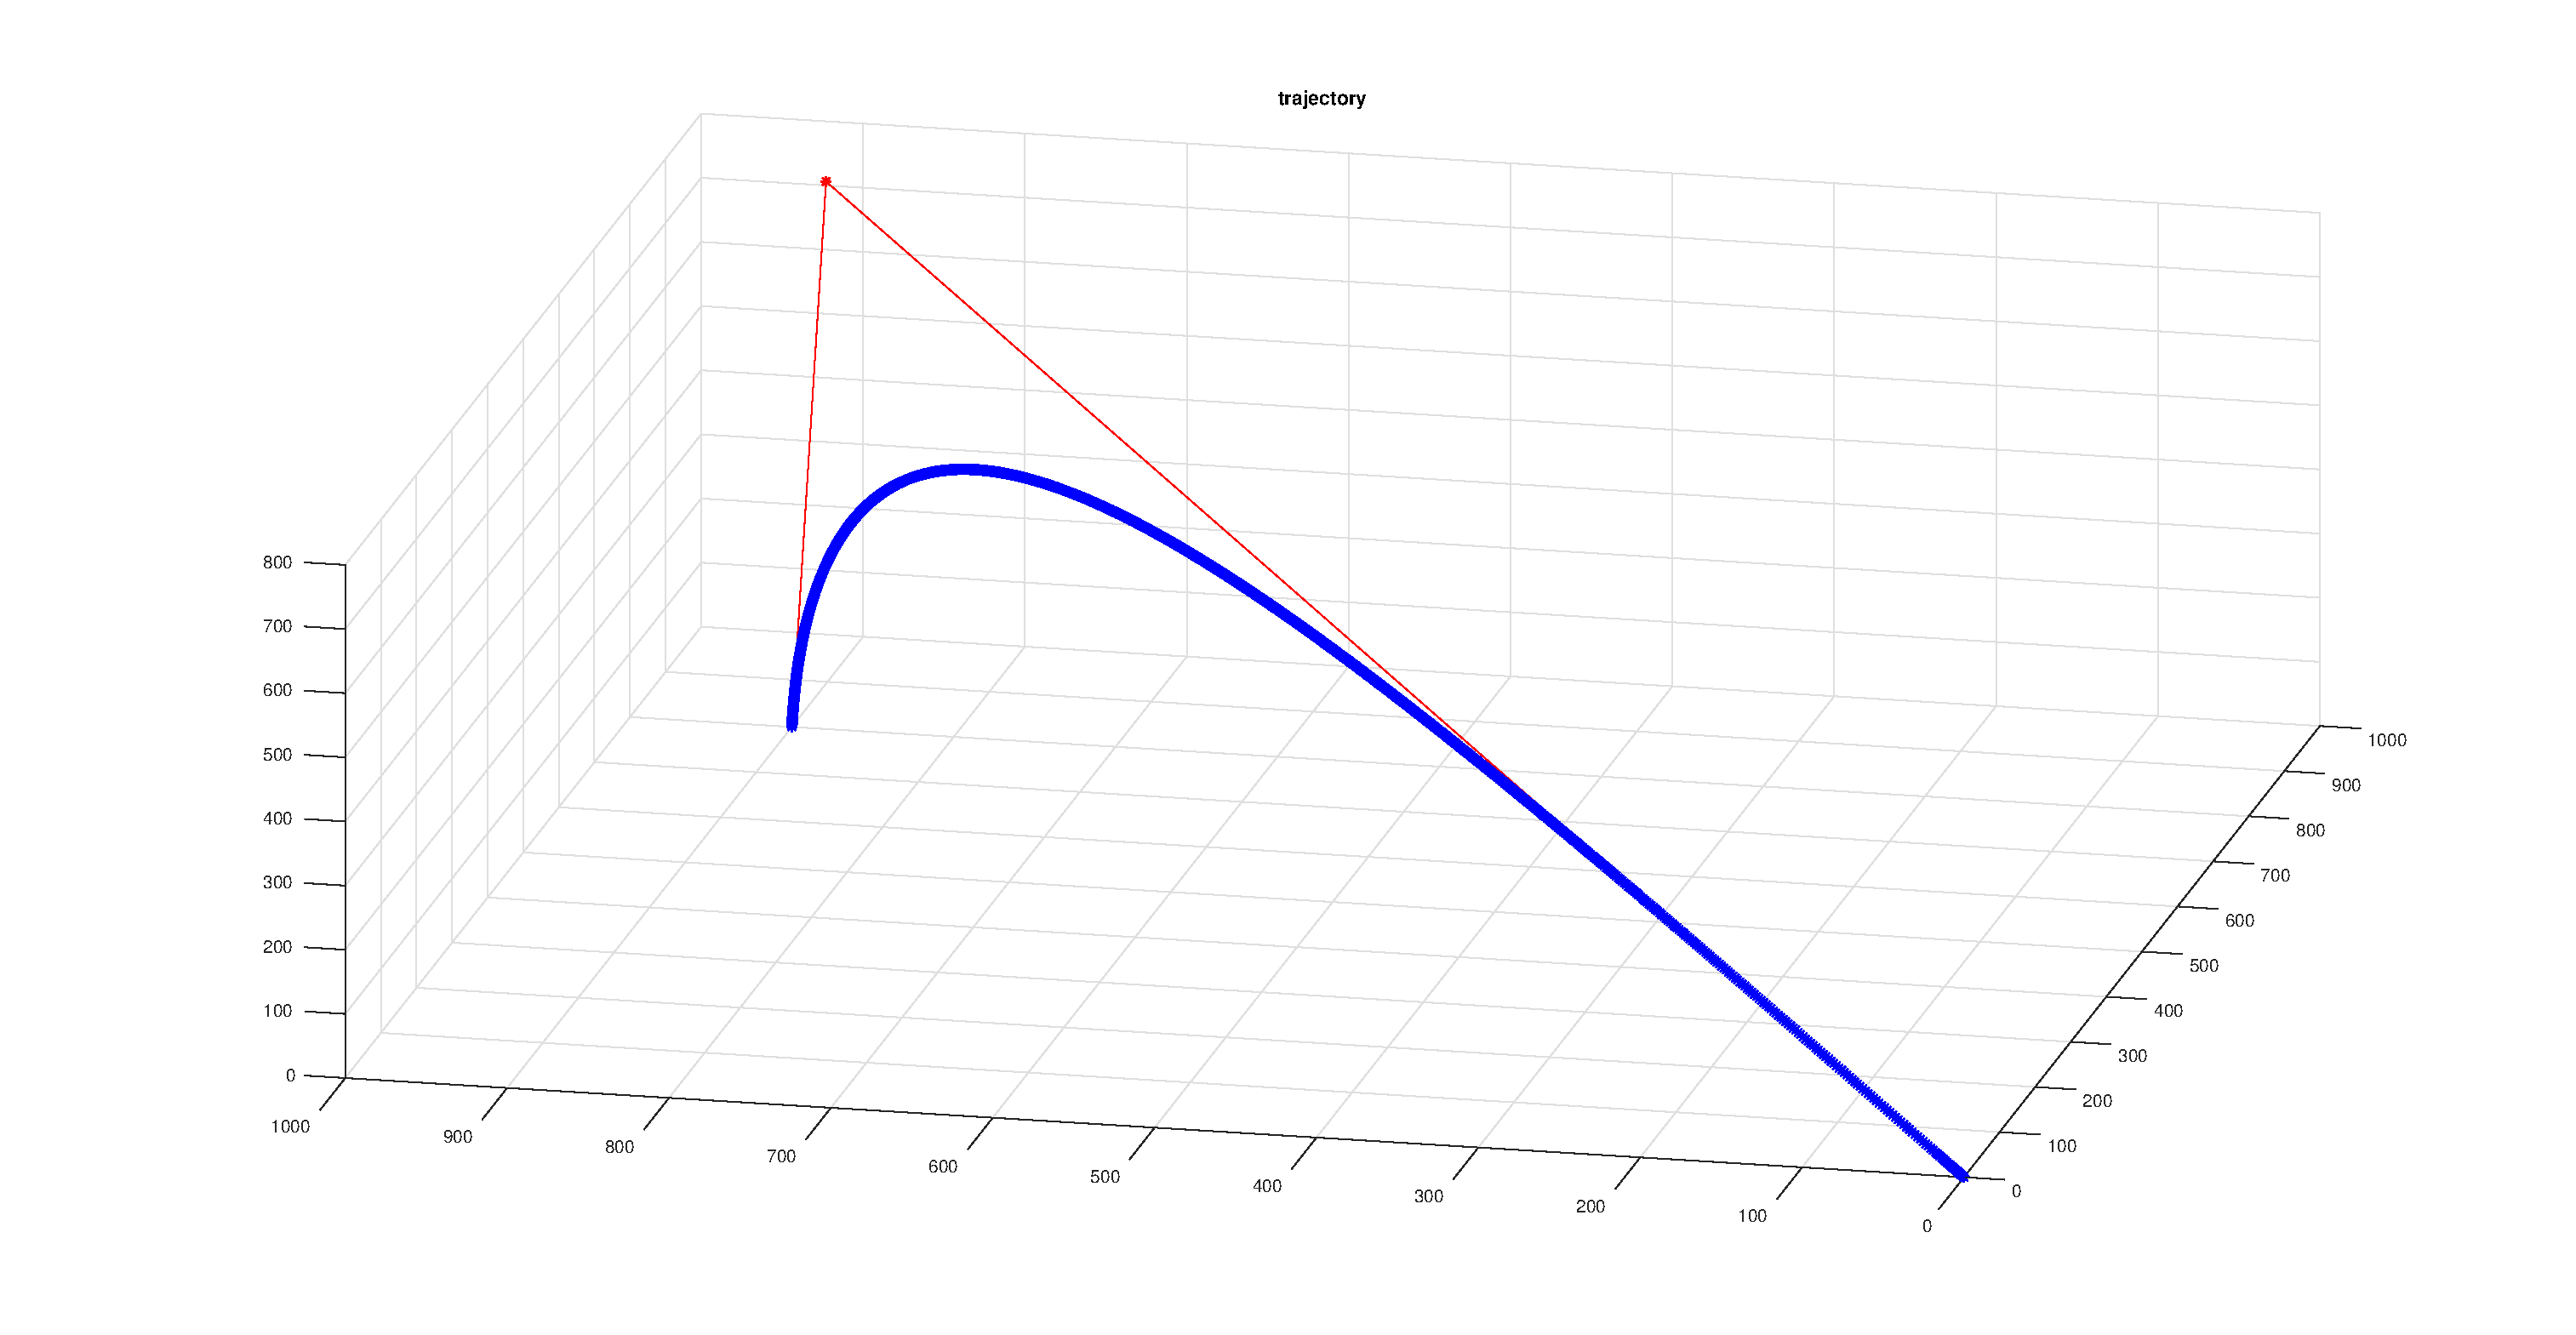
\includegraphics[height=0.6\textwidth]{motion_law_sample_problem_traj}
		\end{minipage}
		\caption[Motion Law Sample Problem]{Motion Law Sample Problem,
		left: problem layout, right: trajectory found}
		\label{fig:motion_law_sample_problem}
	\end{figure}

	\begin{figure}[hbt!]
		\centering
		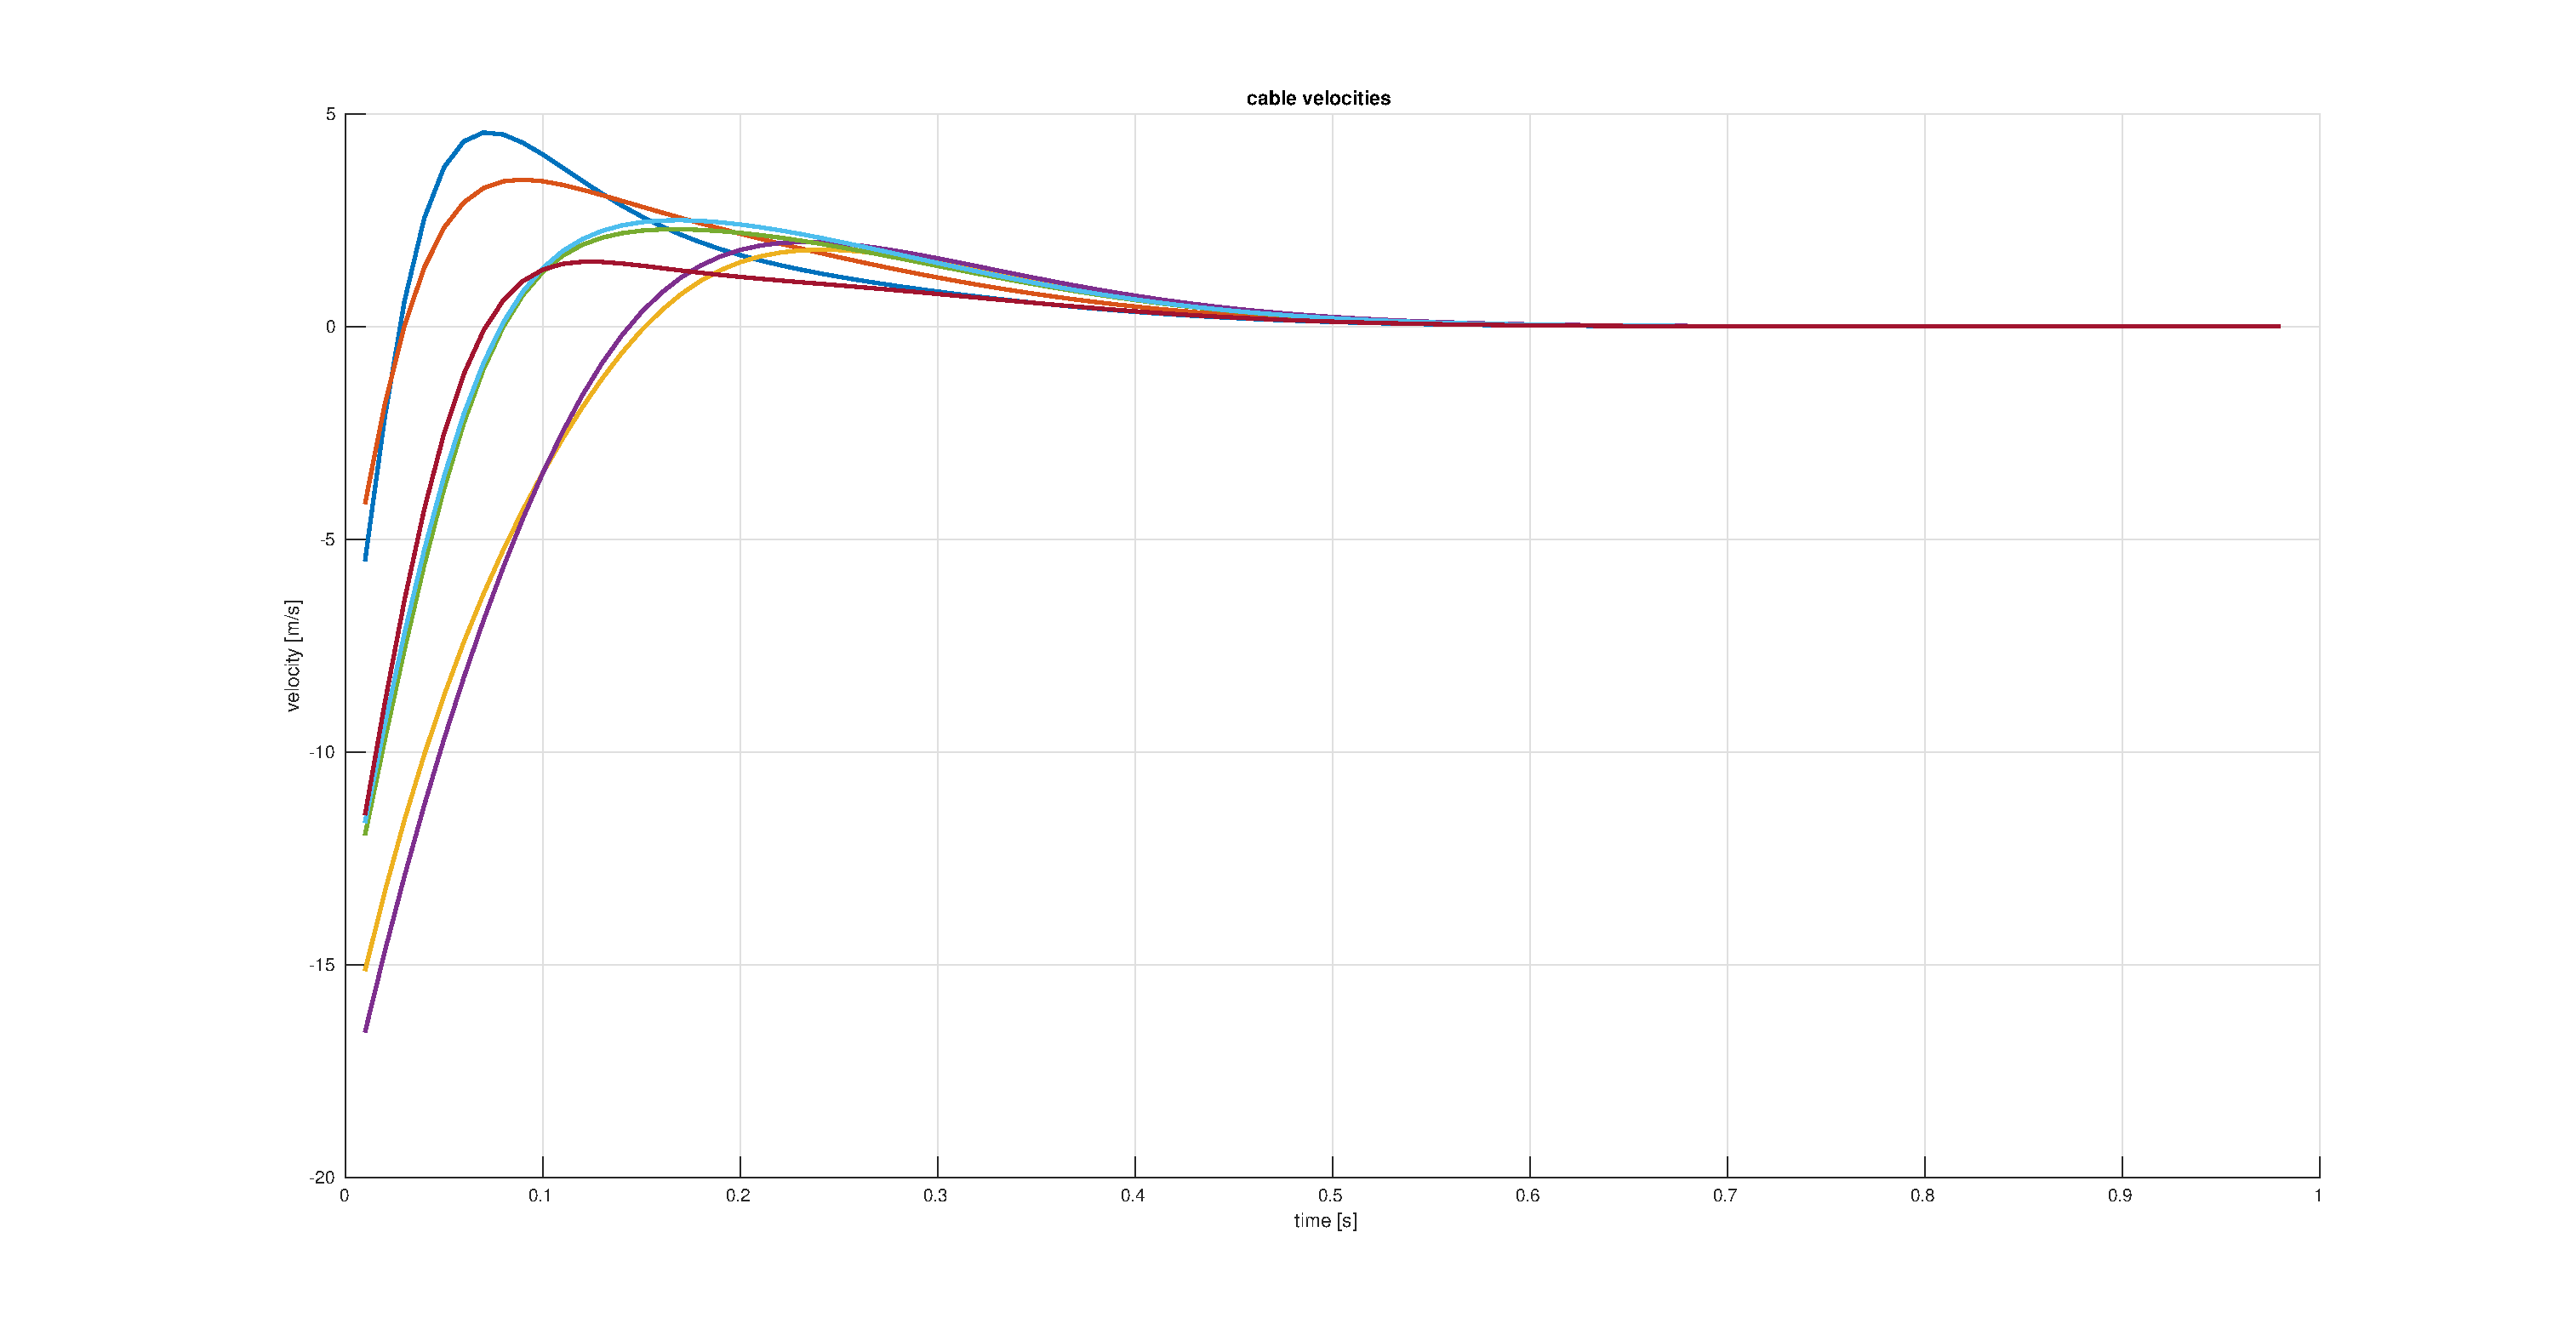
\includegraphics[width=\textwidth]{motion_law_base_velocities}
		\caption{Cable Velocities without Motion Law Scaling}
		\label{fig:cable_velocities_without_motion_law_scaling}
	\end{figure}

	\begin{figure}[hbt!]
		\centering
		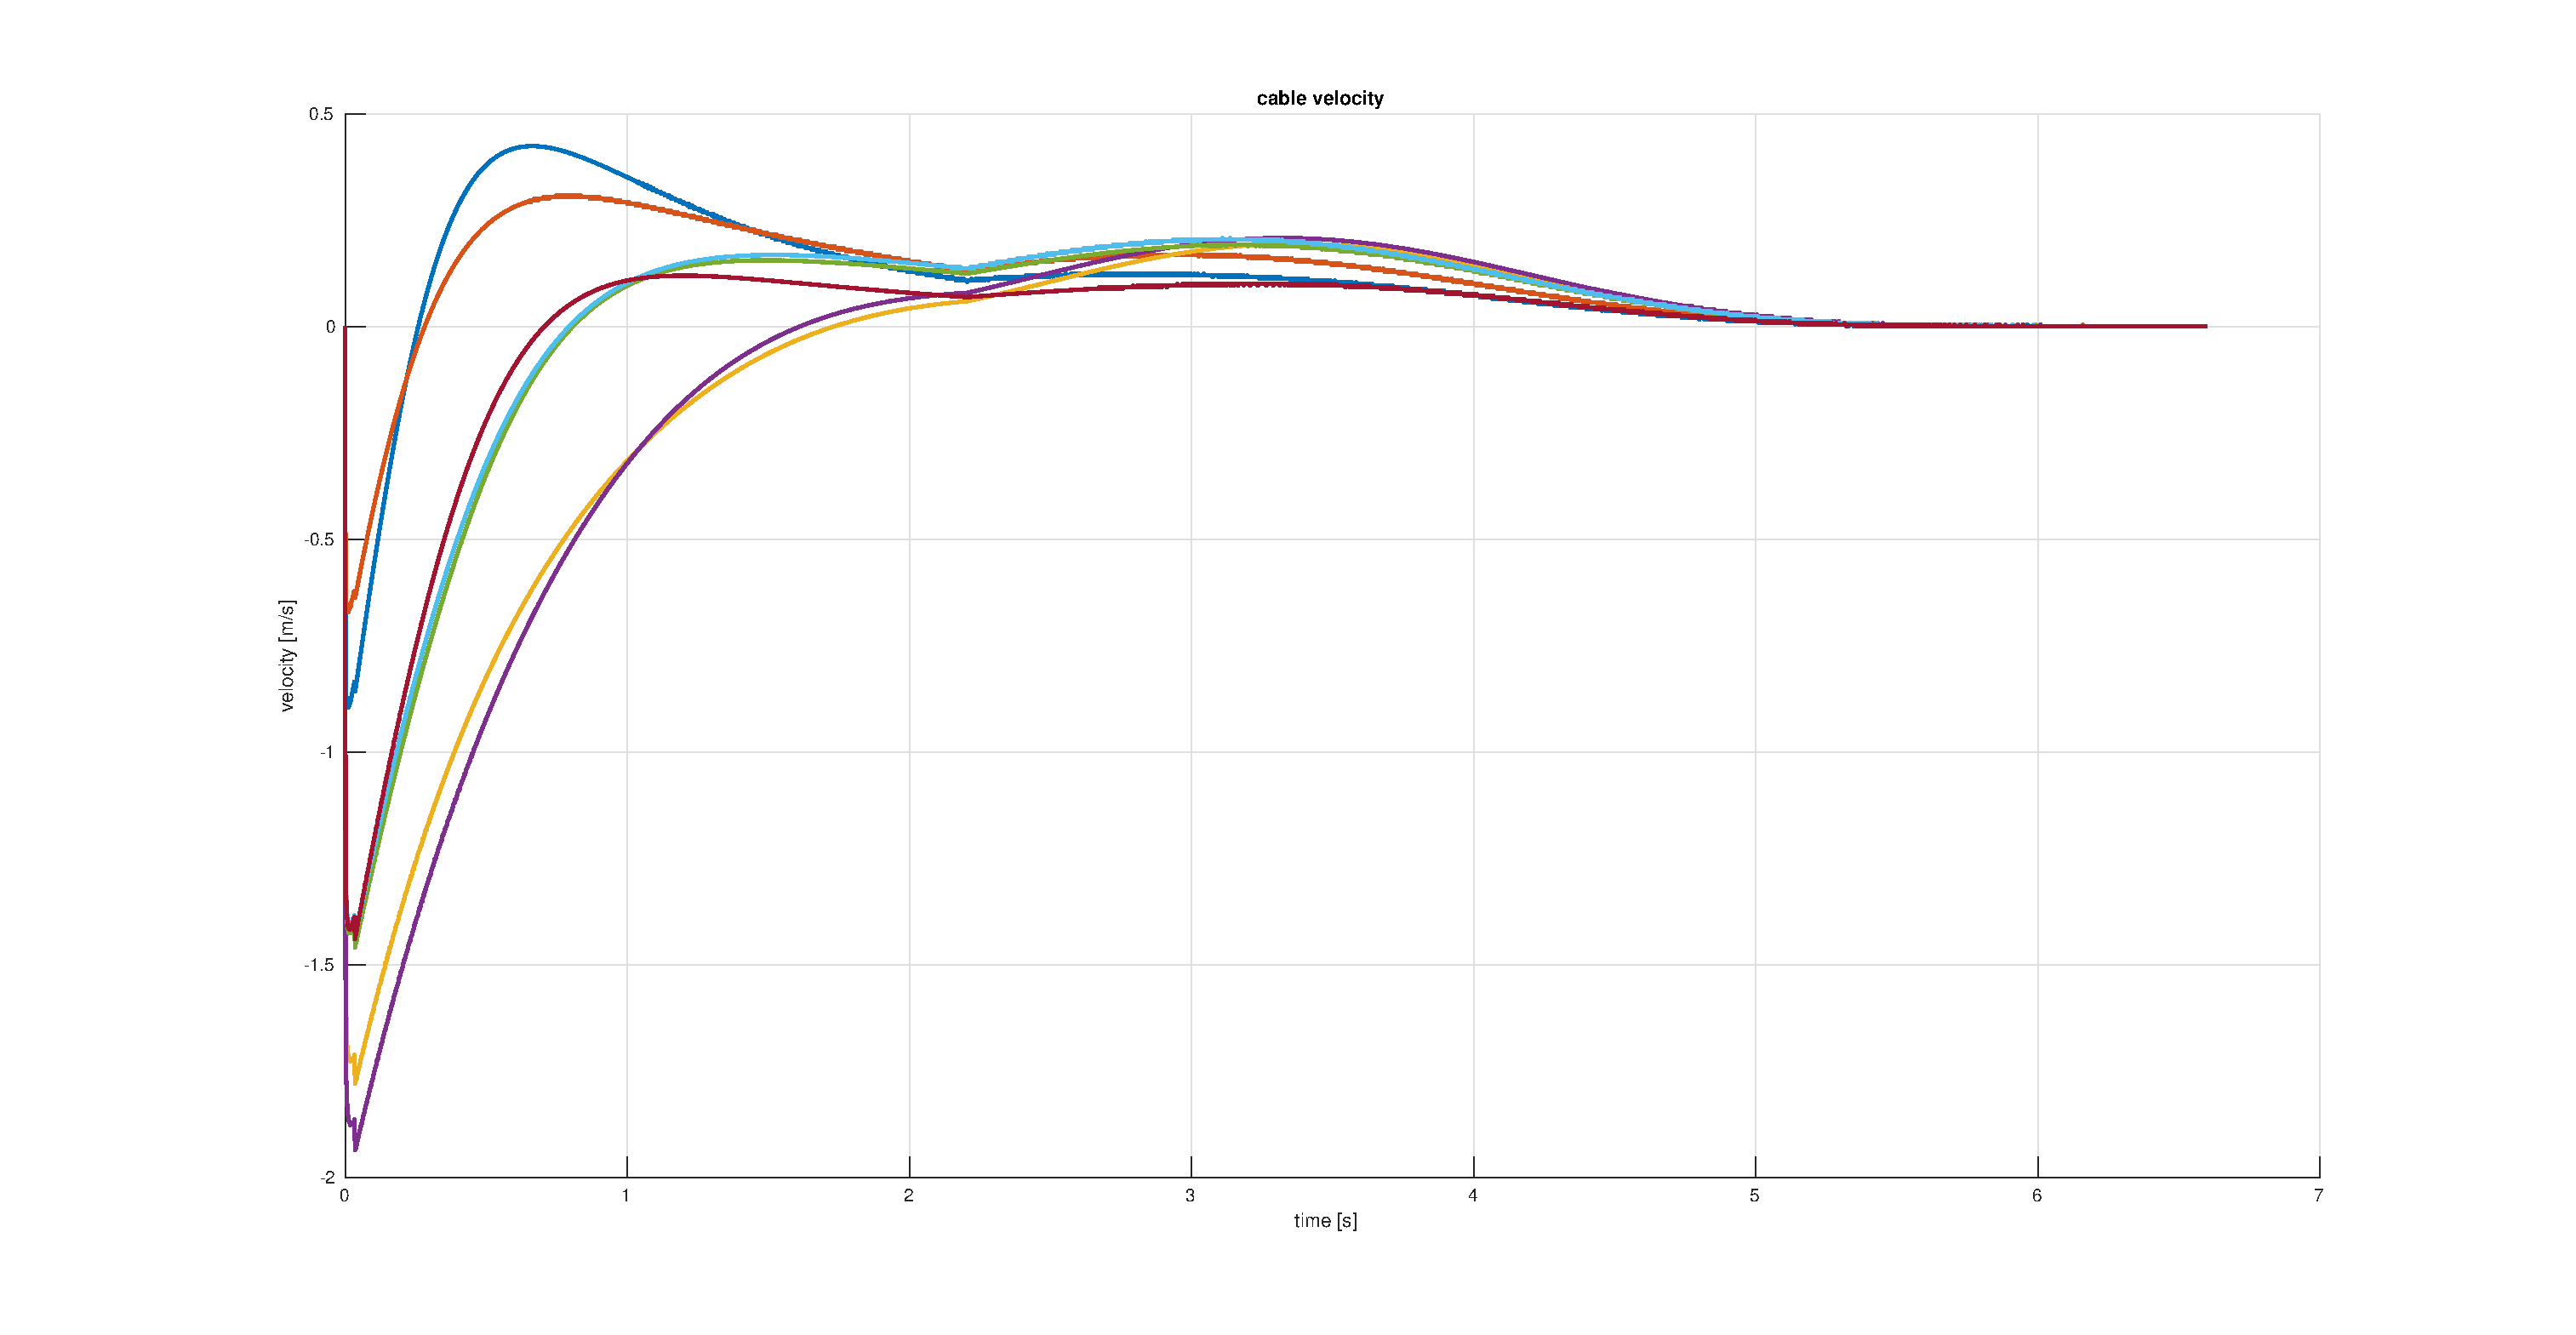
\includegraphics[width=\textwidth]{motion_law_output_velocities}
		\caption{Cable Velocities with Motion Law Scaling}
		\label{fig:cable_velocities_with_motion_law_scaling}
	\end{figure}

	\begin{figure}[hbt!]
		\centering
		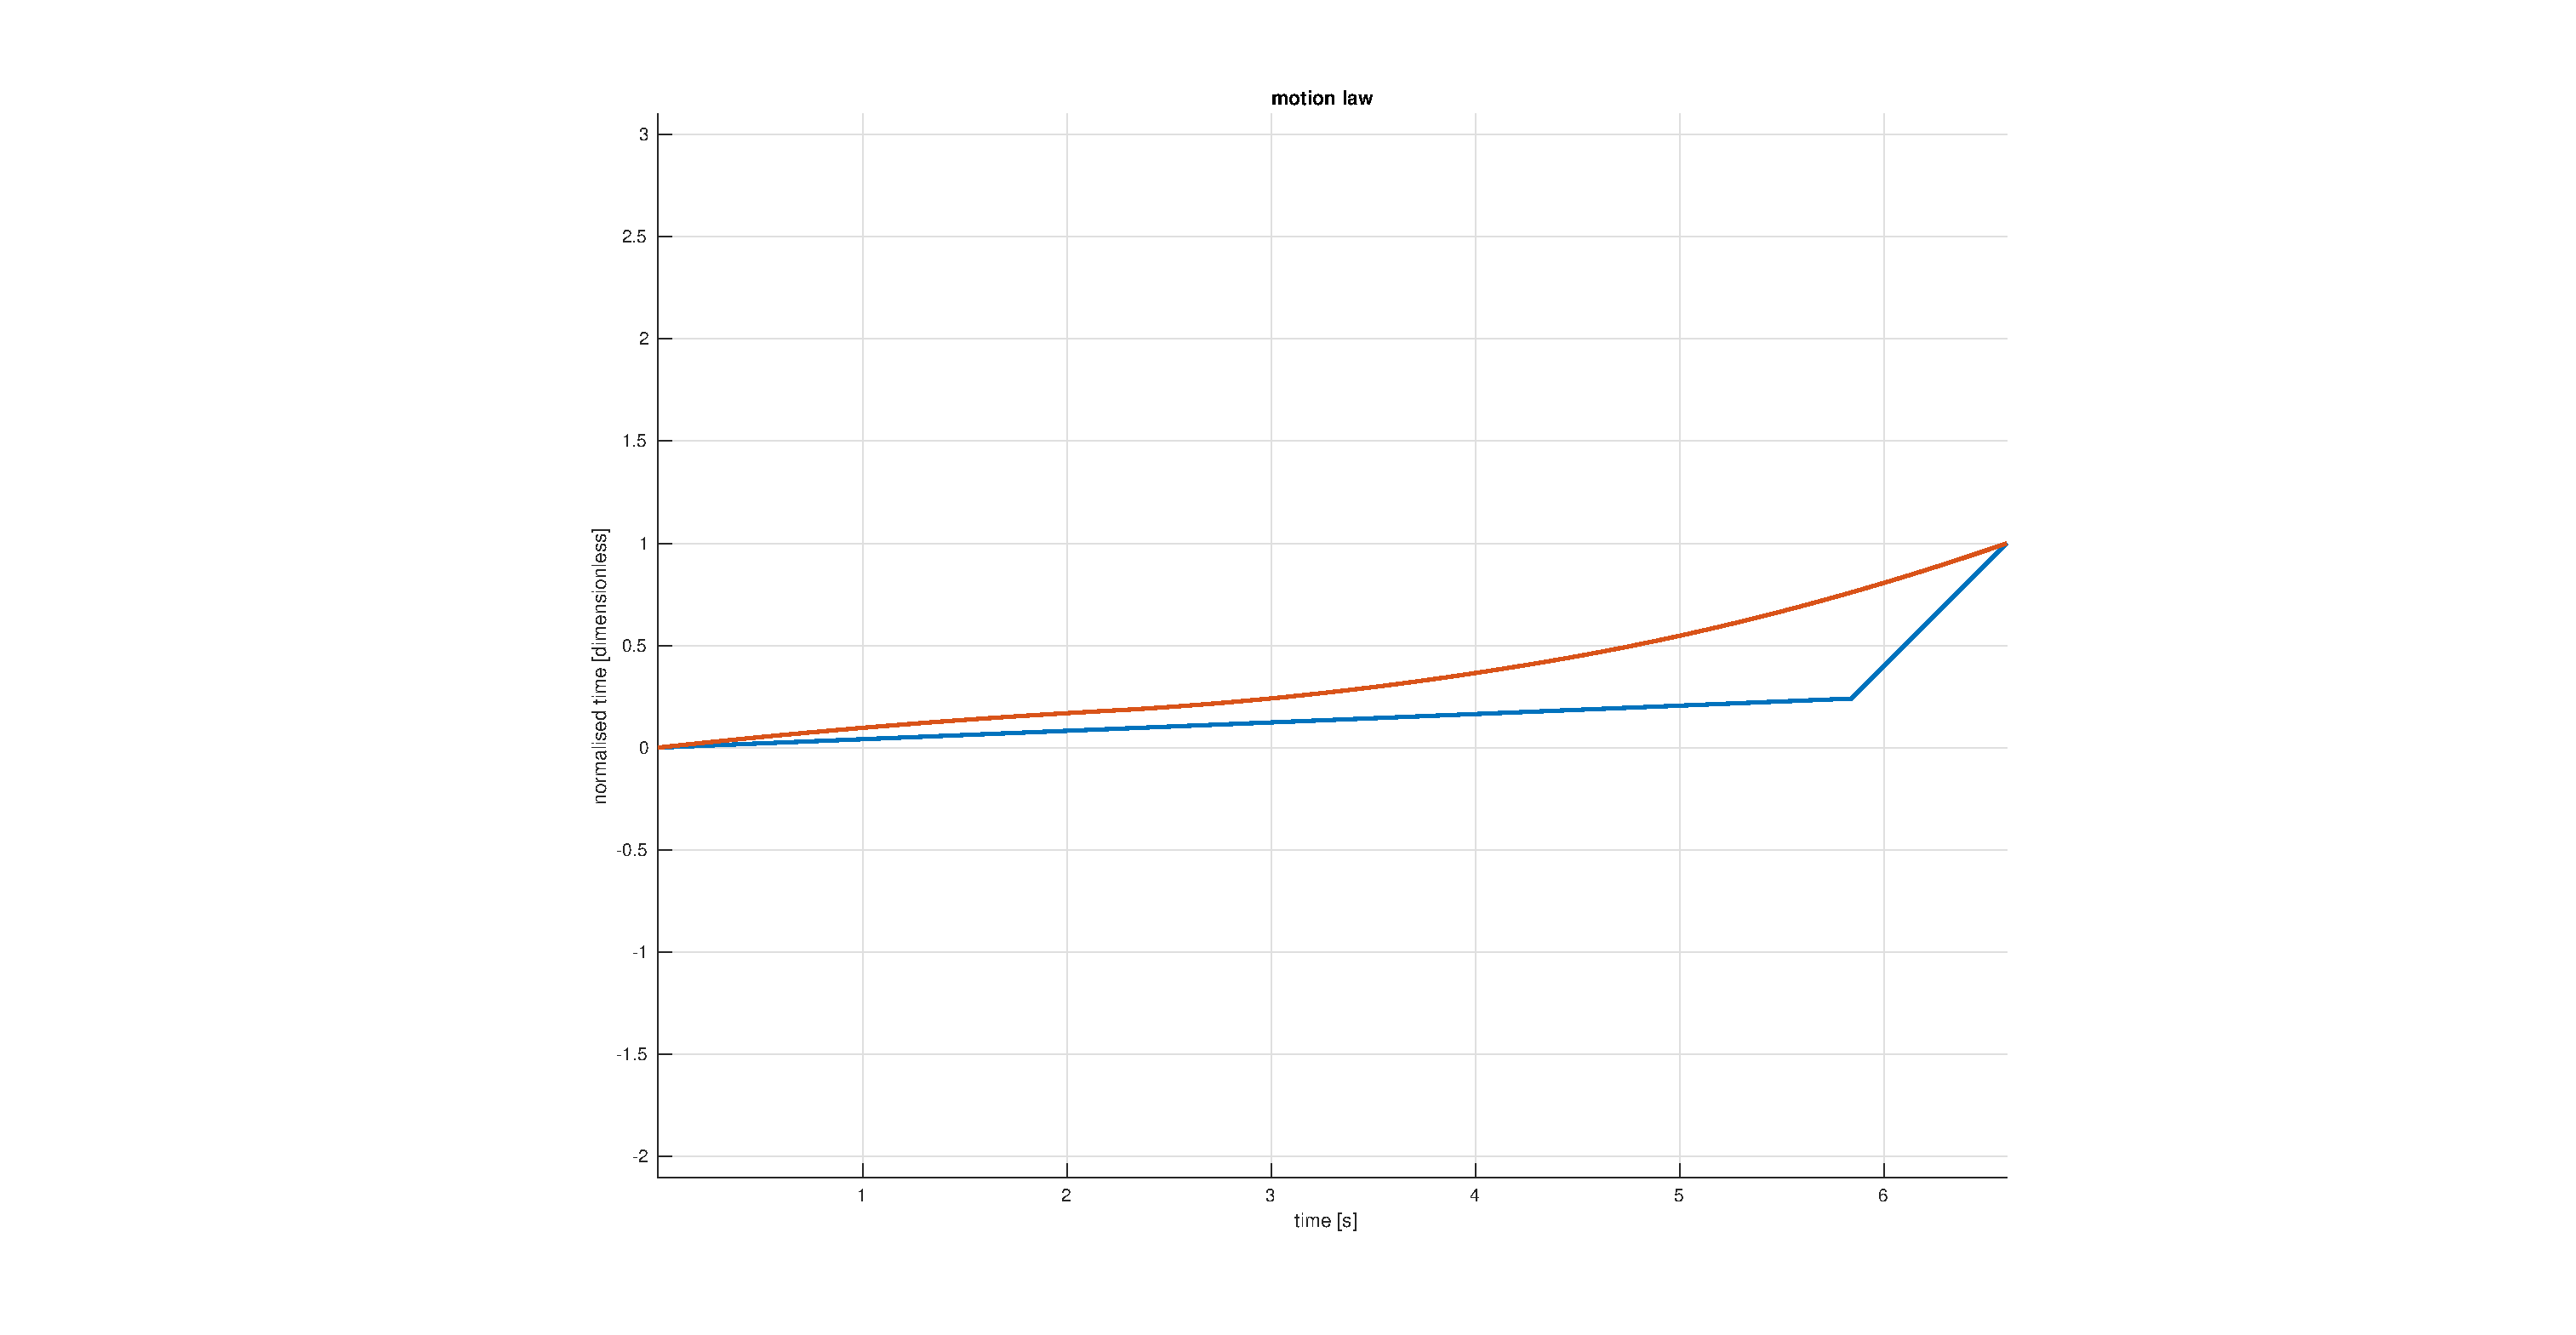
\includegraphics[width=\textwidth]{motion_law}
		\caption{Cable Velocities with Motion Law Scaling}
		\label{fig:motion_law}
	\end{figure}

	The output of the algorithm for this problem is shown in
	Figures~\ref{fig:cable_velocities_without_motion_law_scaling},
	\ref{fig:cable_velocities_with_motion_law_scaling} and~\ref{fig:motion_law}.
	In these figures, the algorithm attempted to find a motion law such that the
	maximum velocity does not exceed $2\si{\meter\per\second}$. For comparison,
	Figure~\ref{fig:cable_velocities_without_motion_law_scaling} shows the case
	where the algorithm is not applied ($\timesym \defeq \timenorm$). As can be
	seen, cable velocities reached up to $15\si{\meter\per\second}$ in this
	case. The motion law generated by the algorithm is reported in
	Figure~\ref{fig:motion_law}. In this figure both the control polygon and the
	B-Spline curve are shown. The output velocities found by applying this
	motion law is shown in
	Figure~\ref{fig:cable_velocities_with_motion_law_scaling}. As can be seen
	from the figurek the motion law succeeds in keeping the cables within their
	velocity bounds.



	\chapter{Experimental Validation}

	\todo{Describe aim of the experiment here}

	\subsection{Experimental Setup}

	\subsection{Results}

	\chapter{Architecture Developed}

	The current chapter gives a brief overview of the architectural design of
	the software.


	\printbibliography{}

\end{document}
